\documentclass[12pt]{article} % JASA requires 12 pt font for manuscripts
%\usepackage{JASA_manu}        % For JASA manuscript formatting
\usepackage{times, asa, url}
\RequirePackage{pdf14}
%\usepackage[bookmarks,linkcolor=black]{hyperref}

% for citations
\RequirePackage{natbib} 
%\usepackage[colorlinks=true, citecolor=blue, linkcolor=blue]{hyperref}
%\newcommand{\citetapos}[1]{\citeauthor{#1}{\textcolor{black}{'s}} }

%\definecolor{Blue}{rgb}{0,0,0.5}

% for figures
\usepackage{graphicx}
%\usepackage{caption}
\usepackage{subfig}
\captionsetup[subfloat]{font=normalsize}
\graphicspath{{figures/}}
\newcommand{\hh}[1]{{\color{orange} #1}}
\newcommand{\al}[1]{{\color{red} #1}}
\newcommand{\aside}[1]{{\color{green} #1}}

% color in tables
\usepackage{color}
\usepackage{colorbl}

% help with editing and coauthoring
\usepackage{todonotes}

% title formatting
% \usepackage[compact,small]{titlesec}
% page formatting
\usepackage[margin = 1in]{geometry}
%\usepackage[parfill]{parskip}

% line spacing
\usepackage{setspace}
\doublespace

% For math typsetting
\usepackage{bm}
\usepackage{amstext}
\usepackage{amssymb}
\usepackage{amsthm}
\usepackage{amsmath}
\usepackage{amsfonts}
\usepackage{multirow}

\newtheorem{proposition}{Proposition}
\newtheorem{theorem}{Theorem}
\newtheorem{definition}{Definition}
\newtheorem{algorithm}[theorem]{Algorithm}

% A few commands to make typing less tedious
\newcommand{\inv}{\ensuremath{^{-1}}}
\newcommand{\ginv}{\ensuremath{^{-}}}
\newcommand{\trans}{\ensuremath{^\prime}}
\newcommand{\E}{\ensuremath{\mathrm{E}}}
\newcommand{\var}{\ensuremath{\mathrm{Var}}}
\newcommand{\cov}{\ensuremath{\mathrm{Cov}}}
\DeclareMathOperator{\tr}{Trace}
\DeclareMathOperator{\rank}{rank}
\DeclareMathOperator*{\argmin}{arg\, min}

\pdfminorversion=4 % Instructed by JCGS submission

\begin{document}

\title{Are you Normal? The Problem of Confounded Residual Structures in Hierarchical Linear Models}
\author{{Adam Loy and Heike Hofmann}
\thanks{Adam Loy is an Assistant Professor in the Department of Mathematics, Lawrence University, Appleton, WI, 54911 (e-mail: adam.m.loy@lawrence.edu); and Heike Hofmann is a Professor in the Department of Statistics and Statistical Laboratory, Iowa State University, Ames, IA 50011-1210.}}

\maketitle

%----------------------------------------------------------------------------------
% Abstract

\begin{abstract}
We encounter hierarchical data structures in a wide range of applications. Regular linear models are extended by random effects to address correlation between observations in the same group. Inference for random effects is sensitive to  distributional mis-specifications of the model, making checks for (distributional) assumptions particularly important.  The investigation of residual structures is complicated by the presence of  different levels and corresponding  dependencies. Ignoring these dependencies leads to  erroneous conclusions using our familiar tools, such as Q-Q plots or normal tests. We first show the extent of the problem, then we introduce the {\it fraction of confounding} as a measure of the level of confounding in a model and finally introduce rotated random effects as a solution to assessing distributional model assumptions. This article has supplementary materials online.
\end{abstract}
{\bf Keywords:} Diagnostic, Multilevel model, Q-Q plot, Random effects distribution

%----------------------------------------------------------------------------------

%----------------------------------------------------------------------------------
\section{Introduction}\label{sec:intro}
%----------------------------------------------------------------------------------
There are a wide range of application areas---from the biological and physical sciences to the social sciences---in which we encounter nested  data.
Whether it is quality control in a manufacturing process that involves the monitoring of a set of components over  time  or students' performances in different schools across the country, analysts have to account for  the correlation between observations in the same group.  Hierarchical linear models, or multilevel models, allow us to do exactly that---but they also require us to make distributional assumptions on both the error terms and the random effects. These assumptions must hold to ensure the validity of the model and all of its resulting conclusions. 
Inference for the fixed effects in linear mixed models is fairly robust against model mis-specification \citep{Butler:1992tx, Verbeke:1997tf}. This is different for random effects \citep{Verbeke:1996va, Verbeke:1997tf}. 
%\hh{XXX why are empirical Bayes estimates relevant? do you need to pull back so much?} \al{XXX The empirical Bayes estimates are relevant because, under normality, the empirical Bayes estimates are the empirical BLUP, and the literature often discuses the EB estimates rather than the EBLUPS}  \hh{- how about: This is different for random effects, which are sensitive to distributional mis-specifications.} 
 \citet{Verbeke:1996va} have shown that the empirical Bayes estimates of the random effects can be severely distorted if the true distribution is not normal; thus, any distributional assumptions must be checked carefully when the random effects are central to the inferential goals.
%\hh{for empirical Bayes estimates of random effects.} are sensitive to distributional mis-specifications \al{ \citep{Verbeke:1996va} }  
%and  therefore have to be checked carefully, especially when they are central to the inferential goals. %such as in the construction of a prediction interval for an unobserved group.
For example, in small area estimation the areas are often modeled as random effects and their distribution is critical in the calculation of prediction intervals when the  within-group sample sizes are small \citep[see][for a cogent discussion of this issue]{Jiang:2001dx}. 

%\hh{XXX how big is the effect of mis-specification? - didn't we have a table with some simulations or were we just talking about making one? } \al{XXX We don't have any simulation results for this right now, and I haven't found any studies in the small area estimation literature yet... but I have found a few citations where they state the need for diagnostics. What is seemingly complicated about a simulation here is the relative lack of agreement on how to create prediction intervals.}
%Another situation where the estimated random effects are of interest is in the analysis of education data. In such a situation, school are typically modeled as random effects, and confidence or prediction intervals are used for comparison to the average school, depending on the question of interest. }

%\hh{XXX Do we really have two approaches? - there are ways to deal with non-normality, but they are expensive. Our approach doesn't provide a solution to non-normality, but it extends the applicability of normal methods by fixing hypersensitivity of standard distributional assessments.  }

Extensions to the standard modeling framework have been suggested to address sensitivity to distributional mis-specifications, such as semiparametric/nonparametric methods \citep{Shen:1999gd, Zhang:2001wo, Ghidey:2004id} or  finite mixtures of normal distributions for the random effects \citep{Verbeke:1996va}. 
We refer the reader to \cite{Ghidey:2010de} for a recent review comparing these methods. 
Semiparametric and nonparametric methods come at a cost: computational complexity is increased, and most of these methods are not widely implemented yet in standard statistical software, thus making them less accessible to the intended audience. 

However, the situation is not quite as dire as it might seem: it turns out that a lot of tests for normality are overly sensitive in assessing deviations of random effects from normality (see discussion in section~\ref{sec:sim-results} and simulation results in the supplement). By addressing the issue of over-sensitivity in evaluating normality, we are able to extend the applicability of normal model methods in a wide range of situations.

%The cost of increased robustness  is increased computational complexity. These methods also have not been widely implemented in statistical software, making them less accessible. %Another approach is to check %this assumption using
%\hh{distributional assumptions with}
 %diagnostic tools. This is the approach on which we focus in this paper.



%\hh{the next paragraph needs a bit of attention. my first reaction as a reviewer would be to say - ok, it's not graphical, but how do those tests do? It distracts a bit from the main intention of the paper. I'd be in favor to remove the paragraph from here and maybe leave it for the discussion that there are other , non-graphical tests. }
%
Several methods to assess the distribution of random effects  have been proposed. Formal tests have been proposed to to detect mixture distributions \citep{Verbeke:1996va} in the random effects and for overall goodness-of-fit tests for both the error terms and random effects \citep{Jiang:2001dx}.
% however, these methods do \hh{not} lend themselves to graphical inspection and have not been implemented in statistical software.
In contrast, the approach on which we focus in this paper is of a graphical nature.

Quantile-quantile (Q-Q) plots \citep{Wilk:1968} are an essential tool for  visually evaluating a specific distributional assumption. In a Q-Q plot we plot the empirical distribution against the expected quantiles from the assumed distribution. The line of identity therefore represents the theoretical distribution and points show quantiles of the empirical distributions. Deviations from the theoretical distribution then manifest themselves as vertical differences between points and the line of identity. This difference is featured in a series of distributional tests. More formally, let $F_n$ be the empirical distribution function (ECDF) based on a sample size of $n$, and $F$ be the hypothesized/true distribution. The absolute difference between the two distribution functions for each sample point, $\left| F_n(x_i) - F(x_i) \right|$, is then the main contributor for the test statistics of the Kolmogorov-Smirnov \cite[KS-test,][]{kolmogorov:1933, smirnov:1948}, the Anderson-Darling \citep[AD-test,][]{adtest:1954}, and the Cram\'{e}r-von-Mises test \citep[CVM-test,][]{cramer:1928, mises:1928}, as shown in table~\ref{tab:tests}.

The KS test uses the maximal  difference, which is shown as the maximal vertical extent between the line of identity and the data points in a Q-Q plot, regardless of the range of the sample.  AD and CVM  are both based on the total area between the line of identity and the empirical distribution function. Compared to the KS  test,  the CVM test downplays the effects in the tails of a (normal) distribution, while Anderson-Darling upgrades the tail effect again due to its additional weighting of $1/\left(F(x)(1 - F(x)\right)$ across the range of the sample. 
\begin{table}
\begin{tabular}{lrl}\hline
Test && Statistic\\\hline\hline
Kolmogorov-Smirnov & $D =$ & $ \sup_{1 \le i \le n} \left | F_n(x_i) - F(x_i)\right|$ \\
Anderson-Darling & $A =$ & $ n \int_{-\infty}^{+\infty} \left | F_n(x) - F(x)\right|^2/\left(F(x)(1 - F(x)\right) dF(x)$\\
Cram\'{e}r-von-Mises & $C =$ & $n \int_{-\infty}^{+\infty} \left | F_n(x) - F(x)\right|^2 dF(x)$ \\\hline
\end{tabular}
\caption{\label{tab:tests} Three prominent tests for normality based on the difference between empirical and hypothesized distribution function. An overview of the performance and power of these tests can be found in \citet{stephens:1974}.}
\end{table}
%
We will be making use of these three tests and the Q-Q plots in our assessment of normality of random effects.

%For hierarchical linear models adjustments for Q-Q plots have been proposed for evaluation of the random effects distribution that include the use of weighted Q-Q plots \citep{Dempster:1985tr, Lange:1989uu, Eberly:2005ee} and confidence bands found from the parametric bootstrap \citep{Schutzenmeister:2012gw}; however, 

In hierarchical linear models the investigation of residual structures is complicated by the presence of  different levels. 
The nested structure of the data is reflected in the residual structure, and just as there is dependence between different levels in the data, we can expect dependencies between different levels in the residual structure. 
%\al{This dependence is most problematic when assessing the distribution of the random effects, and leads to erroneous conclusions from Q-Q plots and other standard tests.}
Q-Q plots, in their weighted \citep{Dempster:1985tr, Lange:1989uu} or unweighted {form},  show univariate distributions, so they are sensitive to distributional deviations due to hidden dependencies, which might lead to erroneous conclusions in evaluating normality, in particular, when the dependency between levels is high due to an unbalanced design. % there is a relatively high degree of shrinkage,  \al{AE wants us to define shrinkage}. 
Data imbalances lead to higher degrees of shrinkage---i.e.~in the prediction of the random effects the mean structure is considered to a higher degree in a trade-off to prevent overfitting of the raw data.
Data imbalances commonly occur in practice, but are often overlooked in the literature. For example, \cite{Eberly:2005ee} explored properties of Lange and Ryan's weighted Q-Q plots for a balanced longitudinal data set and found that, for a properly specified mean structure,  weighted Q-Q plots are effective in  assessing the distribution of the random effects. The same cannot be said for unbalanced data (with properly specified mean structure). %\hh{XXX unbalanced data doesn't san that the  mean structure is not  properly specified} \al{XXX Correct, but Eberly and Thackeray considered the case with a properly specified mean structure. The results of the simulation study presented in the supplemental materials show that their results do not apply to the situation with data imbalances, which is the case that I am trying to make here: that the current tools fail in certain situations with imbalanced data}. 


%Data imbalances lead to higher degrees of shrinkage, and in situations with high degrees of shrinkage weighted Q-Q plots  cannot accurately target the random effect distribution, even if the mean structure is properly specified.


% however, these plots, weighted or unweighted, do not account for the relationship between the predicted random effects and error terms and result in inflated type I error rates. 

%From a graphical perspective the assessment of the assumptions made on the random effects has focused on plotting the empirical distribution of the predicted random effects in quantile plots 

In this paper, we address the problem of distributional assessment due to confounding in residual structures. Section~\ref{sec:ex} illustrates the inadequacy of existing methods based on the predicted random effects. We introduce the concept of rotating the random effects into a reduced-dimensional subspace that is less confounded in Section~\ref{sec:methods}, and illustrate how to obtain rotated random effects at all levels. In Section~\ref{sec:simulation} we evaluate the sensitivity and specificity of tests of normality for the rotated random effects in a simulation study to investigate the behavior of Q-Q plots constructed from the rotated random effects. Finally, we demonstrate how this enables an appropriate graphical assessment of the distributional assumptions in Section~\ref{sec:radon2}. %We conclude with a discussion of how rotated residuals relate to other diagnostic procedures and suggest areas for future investigation.

%\todo[inline]{Should I take out ``and suggest ares for future investigation''?}

%----------------------------------------------------------------------------------
\section{Motivating example}\label{sec:ex}
%----------------------------------------------------------------------------------
%To motivate our discussion
To illustrate the effect of confounding between different levels of residuals, we consider the data set discussed by
 \cite{Gelman:2006ue}. This data set consists of a stratified random sample of 919 owner-occupied homes in 85 counties in Minnesota.  \cite{Gelman:2006ue}  suggest a hierarchical model of the form
%
\begin{equation}\label{eq:radon}
  \log(y_{ij}) = \beta_0 + \beta_1 x_{1ij} + \beta_2 x_{2i} + b_{0i} + b_{1i} x_{1ij}  + \varepsilon_{ij}
\end{equation}
%
where   $\log(y_{ij})$ denotes the  radon measurement (in log $pCi/L$, i.e log picoCurie per liter) for house~$j$ within county~$i$ ($1 \le j \le n_i, 1 \le i \le 85$).
 $x_{1ij}$ is a binary variable describing the level at which the measurement was taken (0 for the basement and 1 for a higher level), and $x_{2i}$ denotes the average soil uranium content for  county~$i$. 
 We assume i.i.d.~normal errors $\varepsilon_{ij} \sim \mathcal{N} (0,\ \sigma^2_{\varepsilon})$  and $\bm{b}_i \sim \mathcal{N}(\bm{0},\ \bm{D})$, where $\bm{D}$ allows for correlation between random effects within the same county $i$. %, $b_{0i}$ and $b_{1i}$. 
 Further, we assume independence between random effects and error terms. 


Figure \ref{fig:map} shows a map of counties in Minnesota. The color shading represents average radon activity in a county. For two counties no data are available. Generally, more southern locations exhibit higher  levels of radon activity. Figure \ref{fig:tc} focuses on the counties of Hennepin (home to Minneapolis) and Winona (home to the city of the same name), plotting radon level by floor level. Radon levels are usually the highest at the basement level of a house. 
%
\begin{figure}[htb]
\centering
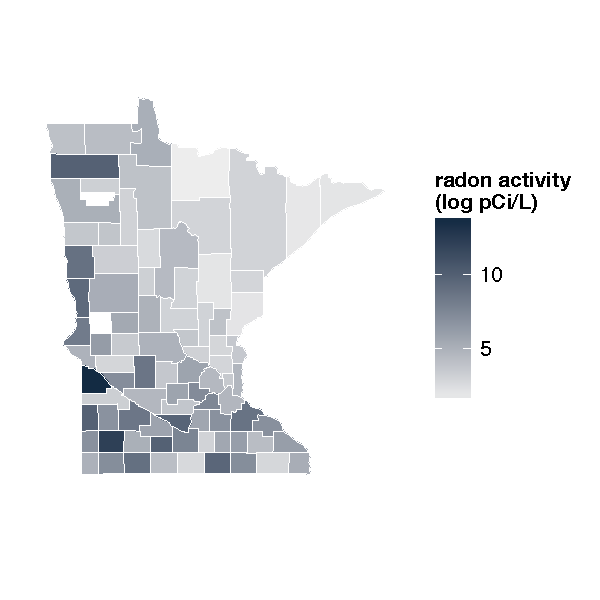
\includegraphics[width=0.5\textwidth]{figures/map.pdf}
\caption{\label{fig:map} Map of the counties in Minnesota. The color shading represents average radon activity (in log $pCi/L$, i.e. log picoCurie per liter).}
\end{figure}
%
\begin{figure}[hbt]
\centering
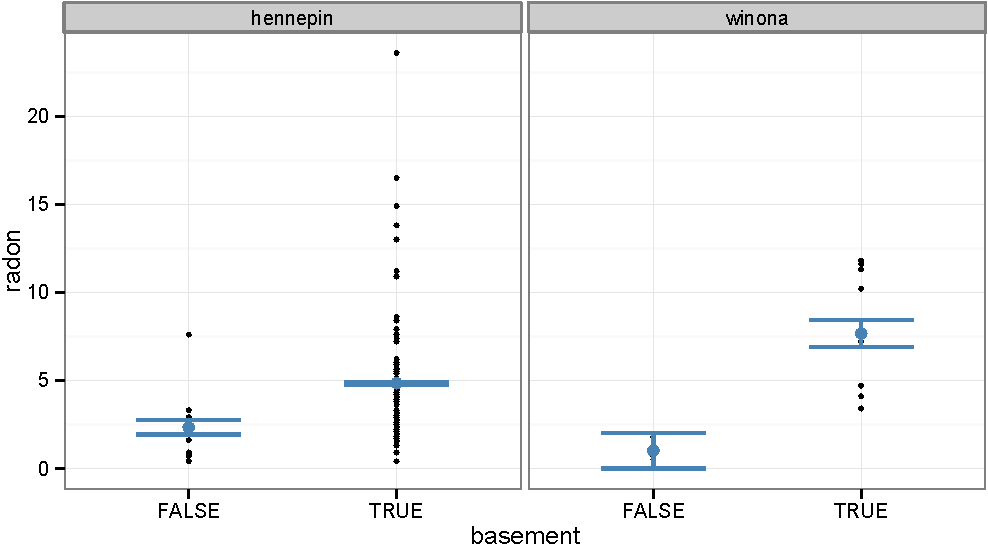
\includegraphics[width=0.7\linewidth]{figures/radon-twocounties.pdf}
\caption{\label{fig:tc} Activity of radon levels for Hennepin and Winona counties at basement (basement = TRUE) or higher in the residence. The bigger points indicate the sample means with 95\% confidence intervals  given by the error bars. Radon levels at the basement level are usually higher.}
\end{figure}
%
The within-county sample sizes, $n_i$, are extremely unbalanced, ranging from one house to 116 houses, with 50\% of the counties having between three and ten houses. Such unbalanced designs are common in applications, and result in a high degree of pooling in the predicted random effects, which results in quantities for many counties that are highly shrunken toward the global mean. It is this high degree of shrinkage that leads to dependence between  predicted random effects and error terms (cf.~eqns.~\ref{eq:resid1} and \ref{eq:resid2}), which in turn can lead us to draw erroneous conclusions for corresponding residual quantities.

\begin{figure}[!h]
	\centering
	  \subfloat[Predicted error terms]{
		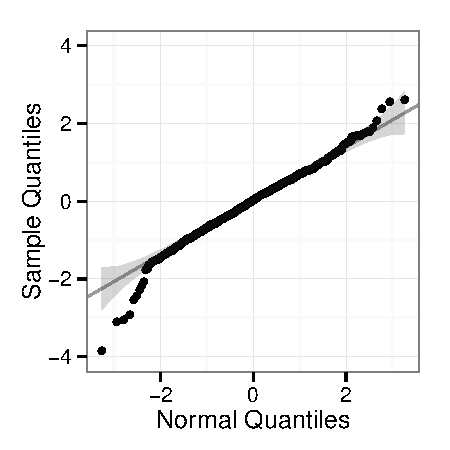
\includegraphics[width=0.33\linewidth]{raw-lev1-qq.pdf}
	   }
	  \subfloat[Random intercepts]{
		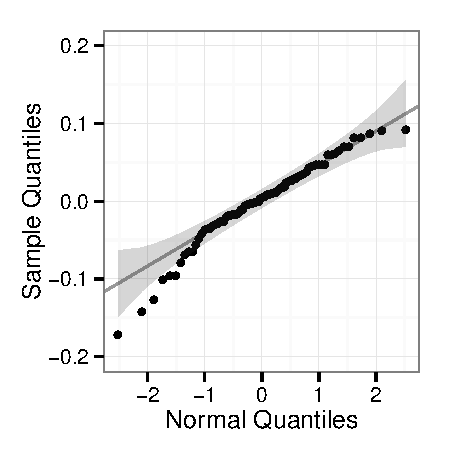
\includegraphics[width=0.33\linewidth]{raw-intercept-qq.pdf}
		}
%	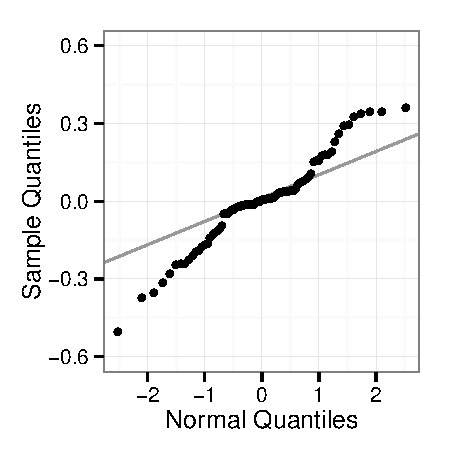
\includegraphics[width=0.32\textwidth]{raw-slope-qq.pdf}
	\caption{\label{fig:qqplots1} Q-Q plots of predicted residuals at different levels %, and random slopes (right) 
	for model~\eqref{eq:radon}. Both plots suggest a deviation of residuals from a normal distribution. Note that random slopes (see figure~\ref{fig:lineup}) exhibit the largest deviation from normality. }
\end{figure}

\begin{figure}[htb]
	\centering
	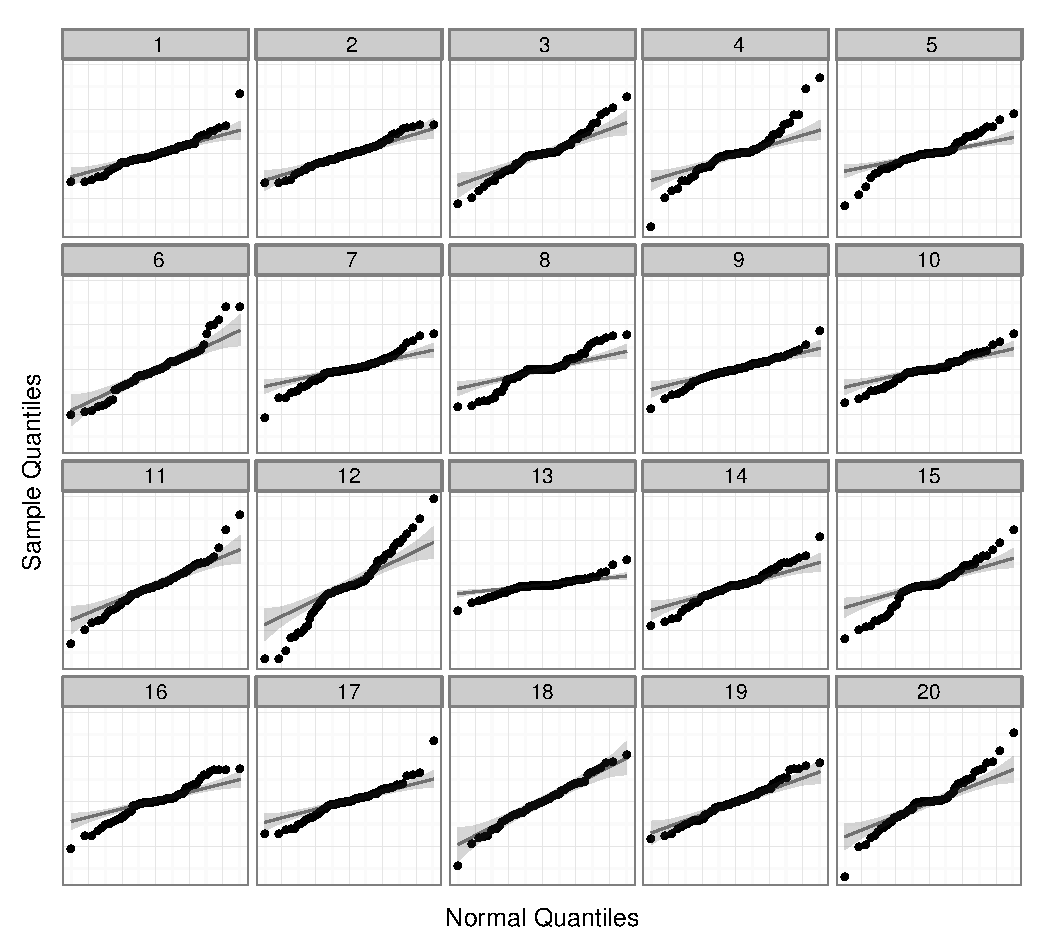
\includegraphics[width=0.9\textwidth]{qq-lineup-std.pdf}%test.jpeg}%lineup-rslope.pdf}
	\caption{\label{fig:lineup} Lineup of normal Q-Q plots for the random slope term in model~\eqref{eq:radon}. The 19 null plots are obtained by simulation from the model. Can you identify the observed Q-Q plot?  In a human subject study 15 out of 23 participants identified panel \#$(3^2+3)$ as the least normal, panel \#$(3^2+7)$ shows the actual data, which none of the participants identified as the least normal. }
\end{figure}


In this example, Q-Q plots (Figure~\ref{fig:qqplots1}) for the residuals show that normality 
seems to be violated for the error terms and random intercepts. But is this cause for concern?
As there is little pooling at the observation level (level 1) we expect the distributional assessment of the error terms to be reliable, but  the high degree of pooling  for the random effects  casts doubt on the reliability of their Q-Q plots. The lineup protocol  \citep{buja:2009} allows us to assess the reliability of the Q-Q plots:
Figure~\ref{fig:lineup} shows a lineup of 20 Q-Q plots for the predicted random slope. The Q-Q plot of the observed random slopes is placed among 19 decoy plots created from parametric bootstrap samples based on model~\eqref{eq:radon} satisfying the normal distribution assumptions. The simulation parameters were set to the maximum likelihood estimates of model~\eqref{eq:radon}. 
If we can identify the real Q-Q plot in the lineup, this provides evidence that the distribution of the observed random slopes is not normal. However, 
the observed Q-Q plot (panel \#$(3^2+7)$) is virtually indistinguishable from the field of null plots. This suggests that the predicted random slopes  from the data do not deviate significantly from model~\eqref{eq:radon}.  Note that an alternative display of the residuals did produce similar results (see appendix~\ref{sec:detrended}).
In practice we must blind ourselves from the true plot for proper use of lineups. In order to not violate this, we did not show the Q-Q plot of random slopes earlier.

What becomes apparent from the lineup is that {\it most} of the null plots in the lineup do not conform to normality. To further investigate the apparent non-normal behavior of predicted random effects we conducted a small simulation study: 
%
We generated 1000 parametric bootstrap samples from model~\eqref{eq:radon} assuming a normal distribution for all random effects, but  varying distributions for  level-1 residuals:  level-1 residuals were generated as normal ($\varepsilon_{ij}^* \overset{iid}{\sim}  \mathcal{N}(\bm{0},\ \widehat{\sigma}^2_\varepsilon)$), heavy tailed ($\varepsilon_{ij}^* \overset{iid}{\sim} (\widehat{\sigma}_{\varepsilon} / \sqrt{3})\, t_3$), and skewed ($\varepsilon_{ij}^* \overset{iid}{\sim} \widehat{\sigma}_{\varepsilon} \, \{ \text{Exp}(1) - 1 \}$).
After fitting model~(\ref{eq:radon}) to each simulated data set, we evaluated the assumption of normality for both the error terms and 
the random effects using the AD, CVM, and  KS tests for normality.  All tests were expected to reject normality at a nominal 5\% rate, however, all type I error rates are hugely inflated for both random effects, which suggests that  an assessment of normality based on the empirical distribution is not possible. 
%
Table~\ref{tab:edf} shows the percentage of these tests rejecting the null hypothesis of normality at the 5\% significance level.
Even when level-1 residuals are normally distributed, normality for random effects is rejected almost half the time (KS-test). For heavy-tailed or skewed level-1 residuals, the distribution of random effects is affected even worse. 
%
%The type I error rates are hugely inflated for both random effects, which suggests, that  an assessment of normality based on the empirical distribution is not possible. 
For example, 84.1\% of the AD tests rejected normality of the random intercept distribution when the level-1 residuals were skewed.
 Use of standardized random effects and the weighted cumulative distribution function proposed by \cite{Lange:1989uu} reduce the type I errors to the nominal level when the error terms are normal, but the type I errors remain inflated for non-normal error terms (this is based on the results of a larger simulation study which we include in Section 1.5 of the supplement).  
Similarly, tests of non-normal random effects often failed to reject if the error terms were normally distributed. %\hh{XXX this doesn't show up in the table - should we include the assessment for the level-1 residuals? - if the tables are merged into one table, there'd be enough space for it.}
This inability to assess distributional assumptions correctly is a symptom typical of confounding between levels of residuals.
%Based on the above results we find that distributional assessment of the predicted random effects is confounded by the distribution of the level-1 residuals.

%The inflated type I error rates for the random effects indicate that the empirical distribution of the random effects cannot be used to assess the assumption of normality. 
In situations with a large amount of pooling, confounding also affects the error terms, which in this particular example were the least affected and did not exhibit signs of deviation from normality.
%In this example we are able to use the empirical distribution to assess normality of  level-1 residuals  as  pooling is minimal at this level. In situations with higher levels of pooling, this may not be the case.

\begin{table}[t]
\centering
\caption{\label{tab:edf} Percentage of tests rejecting the null hypothesis of normality of the predicted random effects at a 5\% significance level when the error terms are normal, heavy tailed, and skewed. The percentages are hugely inflated under each setting compared to the nominal type I error rate. \vspace{.5em}}
\subfloat[Random intercept]{
	\begin{tabular}{l rrr} \hline
	& \multicolumn{3}{c}{Test} \\ \cline{2-4}
	  	&     AD & CVM  & KS \\ \hline
	Normal       	   &	 65.5 & 61.5 &  49.4  \\ 
	Heavy tailed 	   & 89.0 & 87.8 &  78.5  \\ 
	Skewed       	   & 84.1 & 83.0 &  71.5  \\  
	\hline
	\end{tabular}
}
\qquad
\subfloat[Random slope]{
	\begin{tabular}{l rrr} \hline
	& \multicolumn{3}{c}{Test} \\ \cline{2-4}
	  	&     AD & CVM  & KS \\ \hline
	Normal       	  & 87.4 &  86.9 & 81.5  \\ 
	Heavy tailed 	  &	96.5 &	96.7 & 92.7  \\ 
	Skewed       	  &	95.3 &	95.6 & 90.9  \\  
	\hline
	\end{tabular}
}


%\subfloat[Standardized Random intercept]{
%	\begin{tabular}{l rrr} \hline
%	& \multicolumn{3}{c}{Test} \\ \cline{2-4}
%	  	&     AD & CVM  & KS \\ \hline
%	Normal       	   &	 0.048 &	 0.045 &	 0.046  \\ 
%	Heavy tailed 	   & 0.349 & 0.325 & 0.256  \\ 
%	Skewed       	   & 0.520 & 0.487 & 0.399  \\  
%	\hline
%	\end{tabular}
%}
%\qquad
%\subfloat[Standardized Random slope]{
%	\begin{tabular}{l rrr} \hline
%	& \multicolumn{3}{c}{Test} \\ \cline{2-4}
%	  	&     AD & CVM  & KS \\ \hline
%	Normal       	  & 0.039 &	0.041 &	0.048  \\ 
%	Heavy tailed 	  &	0.434 & 0.403 & 0.320  \\ 
%	Skewed       	  &	0.540 & 0.504 & 0.422  \\  
%	\hline
%	\end{tabular}
%}

\end{table}


%\begin{table}[!h]
%\caption{\label{tab:edf} Proportions of tests rejecting the null hypothesis of normality of the predicted error terms and random effects at the nominal .05 significance level. \hh{didn't we want to keep the  background for power? - it should be consistent throughout the paper} Type I error rates are hugely inflated. \vspace{.5em}
%}
%\begin{center}
%\begin{tabular}{l rrr} \hline
%& \multicolumn{3}{c}{Test} \\ \cline{2-4}
% Residual &  AD & CVM & KS \\ \hline
%Error term			 & 0.06 & 0.06 & 0.05\\
%\rowcolor{gray!20} Random intercept 	& 0.48 & 0.46 & 0.35\\
%\rowcolor{gray!20} Random slope 		& 0.75 & 0.75 & 0.68\\
%   \hline
%\end{tabular}
%\end{center}
%\end{table}


In the remainder of this paper we investigate the root of concern that leads to the distributional deviations, and derive residuals that address the issues introduced by pooling, allowing again for a familiar graphical assessment of these distributions.

%----------------------------------------------------------------------------------
\section{Assessing the distribution of the random effects}\label{sec:methods}
%----------------------------------------------------------------------------------

%In this section we develop the rotated random effects and discuss computational and practical issues associated with their use. Before this discussion we present the model and notation used throughout the paper. Additionally, we review the problem of confounding which can be seen in the formulas for the residuals.

%----------------------------------------------------------------------------------
\subsection{Model notation and residuals}\label{sec:resid}
%\subsection{Hierarchical linear models and residuals}\label{sec:resid}
%----------------------------------------------------------------------------------
\noindent
The general stacked representation of the hierarchical linear model is given by
%
\begin{eqnarray}\label{eq:hlm}
 && \bm{y} = \bm{X \beta} + \bm{Z b} + \bm{\varepsilon}, \\ \nonumber
 && \E \begin{bmatrix} \bm{b} \\ \bm{\varepsilon} \end{bmatrix} = \bm{0}, 
 \ \cov \begin{bmatrix} \bm{b} \\ \bm{\varepsilon} \end{bmatrix} = 
  	\begin{bmatrix} \bm{D} & \bm{0}\\ \bm{0} & \bm{R} \end{bmatrix}
\end{eqnarray}
%
where $\bm{y}$ is an $n \times 1$ vector of observed responses, $\bm{X}$ ($n \times p$) and $\bm{Z}$ ($n \times q$) are design matrices, $\bm{\beta}$ is a $p \times 1$ vector of unknown fixed effects, $\bm{b}$ is a $q \times 1$ vector of unobserved random effects, $\bm{\varepsilon}$ is an $n \times 1$ vector of unobserved errors, and $\bm{R}$ and $\bm{D}$ are positive definite covariance matrices.

  %Additionally, it is often assumed that $\bm{\varepsilon}$ and $\bm{b}$ are normally distributed. 
Using this specification, the predicted error terms and random effects are given by 
%
\begin{align}
\widehat{\bm{\varepsilon}} &= \bm{RPy} = \bm{RPZb} + \bm{RP \varepsilon} \label{eq:resid1}\\
\widehat{\bm{b}} &= \bm{DZ}\trans \bm{Py} = \bm{DZ}\trans \bm{PZb} + \bm{DZ}\trans \bm{P \varepsilon} \label{eq:resid2}
\end{align}
%
where $\bm{P} = \bm{V}\inv( \bm{I} - \bm{X} (\bm{X}\trans \bm{V}\inv \bm{X})\inv \bm{X}\trans \bm{V}\inv)$ and $\bm{V} = \bm{ZDZ}\trans + \bm{R}$. 
Equations \eqref{eq:resid1} and \eqref{eq:resid2} reveal that the distributions of the predicted random effects and error terms are interrelated---i.e.,~the distribution of  the predicted random effects depends on the distribution of the error terms and vice versa. As each residual quantity depends on the other, the predicted error terms and random effects are said to be confounded  \citep{HildenMinton:1995wh}.
Additionally, it is easily seen that both \eqref{eq:resid1} and \eqref{eq:resid2} lead to the analysis of correlated and potentially heteroscedastic disturbances as $\var(\widehat{\bm{\varepsilon}}) = \bm{RPR}$ and $\var(\widehat{\bm{b}}) = \bm{DZ}\trans \bm{PZD}$.
The use of standardized residuals can correct the latter issue, but does not address the fact that the residuals are interrelated. While problems may be expected at both levels of the model based on \eqref{eq:resid1} and \eqref{eq:resid2}, we have found that the interpretation of Q-Q plots of the standardized predicted error terms
%
\[
\bm{z}_{\varepsilon} =  \text{diag} \left(\bm{RPR} \right)^{-1/2} \widehat{\bm{\varepsilon}}
\]
%
is unaffected by this interrelationship in the situations that we have considered (see section 1 of the supplement for simulation results). %XXX Reviewer 2 thinks that this may not hold for small cluster sizes, so I am trying to soften the language just a bit. We didn't exhaust all possibilities in our simulation, but the results we have support this statement
 This is not the case with the standardized random effects.  When the degree of pooling is high---as it is in the above radon example, and often is in practice---interpretation of the predicted random effects cannot be separated from the distribution of the error terms. 
%Detailed simulation results documenting the utility of  these residuals are available in the supplementary material. \al{XXX With the comment above, this sentence now seems out of place...}



%----------------------------------------------------------------------------------
\subsection{Rotating the random effects}\label{sec:rotate}
%----------------------------------------------------------------------------------
\noindent
In section~\ref{sec:ex} we have seen that confounding between the different levels of a hierarchical linear model as specified in~\eqref{eq:hlm} leads to erroneous conclusions with respect to the distributions of error terms and random effects. In order to reduce confounding between the levels, we propose an assessment of the residual structure based on an $s$-dimensional rotation of the form $\bm{W}^{\prime} \widehat{\bm{b}}$. This rotation is chosen such that it substantially reduces the amount of confounding. The resulting rotated random effects are standardized, uncorrelated, and homoscedastic residual quantities, which makes them easily assessable with standard tools. In our discussion (and notation) we focus on a two-level model with a single random effect for ease of explanation. However, this approach is not restricted to a two-level model with a single random effect; an extension of the method is given at the end of the section.

%\al{
%
%%In order to correct residuals for the impact of confounding, we propose using a linear transformation, $\bm{W}^{\prime} \widehat{\bm{b}}$, of the predicted random effects that substantially reduces the amount of confounding. This approach enables the construction of Q-Q plots which are arguably the most familiar graphical depictions for distributional assessment. Additionally, the rotation of the random effects yield residuals that are standardized, uncorrelated, and homoscedastic.
%
%To begin, we will consider a two-level random intercept model, a special case of model \eqref{eq:hlm}. When assessing the plausibility of normality of the random intercept it is tempting to simply construct a Q-Q plot of the predicted random effects; however, we know that this approach is flawed. To address the issue of confounding, we propose the construction of Q-Q plots of an $s$-dimensional rotation of the random intercept of the form $\bm{W}^{\prime} \widehat{\bm{b}}$ that  substantially reduces the amount of confounding. The rotated random intercepts are easily plotted and are standardized, uncorrelated, and homoscedastic residual quantities. While we focus our discussion (and notation) on a two-level model with a single random effect for ease of explanation, we describe how to extend this method at the end of this section.
%}
%\al{
%First, we must define the \emph{fraction of confounding} for the random effects, which is minimized in the result below. This definition generalizes the fraction of confounding proposed by \cite{HildenMinton:1995wh}. 

As a measure of confounding between the levels of a hierarchical model of the form (2), we introduce FC, the {\it fraction of confounding}:
\begin{definition}[Fraction of confounding] 
Let $\bm{b}$ denote a vector of $q$ random effects and $\widehat{\bm{b}}$ its predictions as defined in \eqref{eq:resid2}. For a full rank matrix $\bm{W} \in \mathbb{R}^{q \times s}$, where $ s \le q$, the fraction of confounding in the $s$-dimensional space spanned by $\bm{W}$ is defined as 
\begin{equation}\label{eq:fc2}
\mathrm{FC}(\bm{W}; \widehat{\bm{b}}) = \frac{1}{q} \tr\left( \left(\bm{W\trans B W} \right)\ginv \left(\bm{W\trans A W}\right) \right),
%\dfrac{1}{\ell} \displaystyle{\sum_i} \frac{\bm{v_i}\trans \bm{A} \bm{v_i}}
%		{\bm{v_i}\trans \bm{B} \bm{v_i}}.
\end{equation}
where $\bm{B}$ is the covariance structure of $\bm b$, $\bm{B} = \var(\widehat{\bm{b}})$, and $\bm{A}$ is the conditional covariance structure of  $\widehat{\bm{b}}$ given $\bm{b}$,  i.e. $\bm{A} = \var(\widehat{\bm{b}} | \bm{b} )$.
\end{definition}
\noindent
Note that both $\bm{A}$ and $\bm{B}$ are  positive semidefinite matrices. While it is not immediately obvious that FC % $\tr\left( \left(\bm{W\trans B W} \right)\ginv \left(\bm{W\trans A W}\right) \right)$ 
is well defined,  the following discussion will clarify this point. %XXX This was recommended by reviewer \#2 but it seems forced...

Generally, $\text{FC} \in [0,1]$, where 1 indicates that, due to confounding, the predicted random effects contain no information in addition to that found in the error terms, while a value of FC = 0 indicates that no confounding is present. 

Notice that if $\bm{W}$ is the identity, then \eqref{eq:fc2} measures the fraction of confounding in the original vector of predicted random effects as proposed by  \cite{HildenMinton:1995wh}. %As noted by a reviewer, t
There are many ways of defining a fraction of confounding using different symmetric functions of the relative eigenvalues of $\bm{WAW}\trans$ to $\bm{WBW}\trans$. Here, we chose the trace of the ratio to generalize the results in \cite{HildenMinton:1995wh}. %, but other symmetric functions could be investigated. 
Another natural choice for a symmetric function is  the ratio of the determinants. This function leads to an optimization problem referred to as the ``determinant ratio'' problem, which is equivalent to the ``ratio trace'' problem we consider here \citep{Fukunaga:1990}.
The ratio of the traces (called the ``trace ratio'' problem) on the other hand, does not have a  closed form solution to the analog of the optimization problem we discuss below \citep[cf.,][]{Jia:2009ux}. 


%As outlined above, the confounded nature of the predicted random effects renders graphical explorations of these residuals inadequate for the assessment of distributional assumptions. 
%
%In order to graphically assess the distributional assumption made on the random effects we propose a reduced set ($s$-dimensional rotation) of rotated random effects, $\bm{W}^{\prime} \widehat{\bm{b}}$, by minimizing the amount of confounding present.  


For any given dimension $s$, the linear combination $\bm{W} \in \mathbb{R}^{q \times s}$ that minimizes \eqref{eq:fc2} also minimizes
%
\begin{equation}\label{eq:minimize}
J_1(s) = \tr\left( \left(\bm{W\trans B W} \right)\inv \left(\bm{W\trans A W}\right) \right)
%\displaystyle{\sum_i} \frac{\bm{v_i}\trans \bm{W} \bm{A} \bm{W}\trans \bm{v_i}}
%		{\bm{v_i}\trans \bm{W} \bm{B} \bm{W}\trans \bm{v_i}}
\end{equation}
%
Mathematically, this problem is solved using the generalized eigenvalue decomposition
%
\begin{equation}\label{eq:geigen}
	\bm{Aw}_k = \gamma_k \bm{Bw}_k
\end{equation}
%
where $\gamma_k$ and $\bm{w}_k$ are the $k$-th smallest eigenvalues and eigenvectors, respectively \citep{Fukunaga:1990}. 
%thus, $\bm{W}^*$ consists of the eigenvectors associated with the $s$ smallest eigenvalues. 
Simultaneous diagonalization of $\bm{A}$ and $\bm{B}$ can be used to solve this problem, given that the kernel of $\bm{B}$ is a subspace of the kernel of $\bm{A}$ \citep{deLeeuw:1982to}.
Equivalent to that, we have to show that the difference $\bm{B} - \bm{A}$ is nonnegative definite:
\[
	\bm{A} =  \var(\widehat{\bm{b}} | \bm{b} ) = \bm{RPZDZ}^\prime \bm{PR}
\]
and
\[
	\bm{B} = \var(\widehat{\bm{b}}) =  \bm{RPR} =  \bm{RPVPR}  = \bm{RPRPR} + \bm{RPZDZ}^\prime\bm{PR},
\]
so $\bm{B}-\bm{A} =  \bm{RPRPR}$ is nonnegative definite.

%
%\cite{deLeeuw:1982to} shows that simultaneous diagonalization of $\bm{A}$ and $\bm{B}$ solves this generalized eigenvalue problem if the null space of $\bm{B}$ is a subspace of the null space of $\bm{A}$, for which a sufficient condition is that $\bm{B} - \bm{A}$ be nonnegative definite. In our problem 
%\[
%	\bm{A} =  \var(\widehat{\bm{b}} | \bm{b} ) = \bm{RPZDZ}^\prime \bm{PR}
%\]
%and
%\[
%	\bm{B} = \var(\widehat{\bm{b}}) =  \bm{RPR} =  \bm{RPVPR}  = \bm{RPRPR} + \bm{RPZDZ}^\prime\bm{PR},
%\]
%so $\bm{B}-\bm{A} =  \bm{RPRPR}$ is nonnegative definite.

Simultaneous diagonalization of $\bm{A}$ and $\bm{B}$ requires $\bm{W}$ to be $\bm{B}$-orthogonal, so the optimal $\bm{W}$ is found to be
%
\begin{equation}\label{eq:optimw}
	\bm{W}^*(s) = \argmin_{ 
%\begin{scriptsize}
%	\begin{cases}
      \bm{W} \in \mathbb{R}^{q \times s}, \ \ 
      \bm{W\trans B W} = \bm{I}
%	\end{cases}
%\end{scriptsize}
	} 
\tr\left( \bm{W\trans A W} \right).
\end{equation}
%
The rotated random effects are then given by $\bm{W}^{*\prime} \widehat{\bm{b}}$, which are standardized, uncorrelated, and homoscedastic (see the appendix for a proof and a detailed overview of simultaneous diagonalization). % In the interest of space we have relegated a detailed overview of the procedure used to simultaneously diagonalize $\bm{A}$ and $\bm{B}$ to the appendix (XXX supplementary materials?) 
Simultaneous diagonalization will be familiar to many as the standard canonical transformation used in multivariate regression. % (XXX this was pointed out by the AE, is this OK to add?).


\paragraph{Selection of the dimension of the subspace}
 spanned by the rotated residuals is central to our proposed method. Ideally, we would select the dimension such that the fraction of confounding is reduced to zero; however, this is not realistic in practice. Alternatively, we propose choosing the dimension that provides a substantial reduction in the fraction of confounding. As our ultimate objective is an assessment of the distribution, we must balance this reduction in the fraction of confounding with the loss in power of a test of the empirical distribution function % (e.g., the Anderson-Darling test for normality) 
 associated with dimension reduction. To guide this choice we suggest plotting the reduction in the fraction of confounding against the reduction in dimension, which is similar to the concept of a scree plot used to select the number of principal components. %\hh{A name for this scree-like plot would be good ... talus is a synonym to scree ... talus plot? - or elbow plot?} 
 
 To illustrate the use of this plot we simulate two simple random intercept models with a group-level predictor:   model $M1$ has 40 groups of 30 observations and 10 groups of 5 observations;   model $M2$ also has 50 groups, with group sizes determined as random draws from either a Poisson(30) distribution (40 groups) or a Poisson(5) distribution (10 groups). %\todo[inline]{These two models are very similar. Go to a more extreme in the second model?}
 Figure~\ref{fig:elbow} shows two examples of such plots constructed for the simulated models. For neither model the fraction of confounding for a one-dimensional reduction decreases because this {one-dimensional reduction} simply adjusts for the rank deficiency of the covariance matrix, which can be thought of in terms of adjusting for the effective degrees of freedom. Both figures have an ``elbow'' in the plot corresponding to a reduction in the dimension of the subspace of 11; thus we would choose $s = 39$. Additionally, we see that the elbow in the plot for model $M2$ is less pronounced. This occurs because the groups sizes are less balanced so the difference between the large and small group sizes is reduced. 
 
At first it may be mildly surprising that so few dimensions need to be excluded in this example, but both the group size and variability factor in to the fraction of confounding. Consequently, if there are relatively few small groups, more variable groups, or some combination of the two, then the fraction of confounding is reduced most by reducing the impact of these groups. As a reviewer pointed out, this is quite like the use of dropping the last few PCA dimensions to reduce the impact of outliers.
 
 
 
% \al{Talk about the differences here and why I chose these examples. Also talk about the loss of 1 d.f. More discussion here.}
%
\begin{figure}[htb]
	\centering
	 \subfloat[Model $M1$]{
		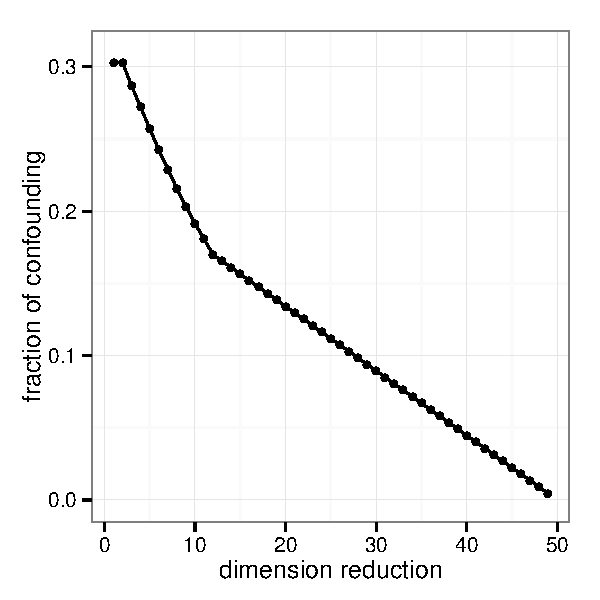
\includegraphics[width=0.4\linewidth]{elbow1.pdf}
		}
	  \subfloat[Model $M2$]{
		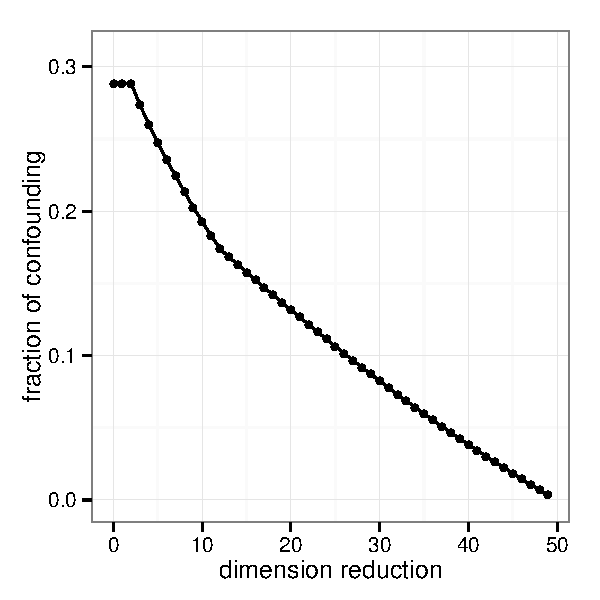
\includegraphics[width=0.4\linewidth]{elbow2.pdf}
		}	
	\caption{\label{fig:elbow} Plots of the fraction of confounding for each reduction in the dimension of subspace spanned by the rotated random intercepts from two simulation models. Model $M1$ has 50 groups: 40 groups of size 30, and 10 groups of size 5. Model $M2$ has 50 groups with group sizes determined as random draws from either a Poisson(30) distribution (40 groups) or a Poisson(5) distribution (10 groups). Based on these plots we  choose $s = 39$, corresponding to a dimension reduction of 11.}
\end{figure}


%%First, we must consider the selection of the dimension of the subspace spanned by the rotated residuals, $s$---that is, the length of the resulting transformed residual vector. 
%For the level-1 residuals \cite{HildenMinton:1995wh} suggests using $s = \rank(\bm{B})$;
%%One choice is $s = \rank(\bm{B})$, which aligns with the suggestion given by \cite{HildenMinton:1995wh} for the level-1 residuals. 
%%This selection has the advantage that it works in all situations, but the disadvantage that the fraction of confounding will \al{often} not be \al{significantly} reduced. 
%An alternative approach is to select $s$ based on the desired reduction in the fraction of confounding. \hh{You need to sell this point a bit more - what is the theoretical advantage of going down on the number of residuals? -- if the approach is to get FC down as much as possible, but have s at least 30, it is always going to end up at 30. What I still don't understand is that the minimization is not taking care of the percent of confounding to a higher degree, because that's really what it was supposed to do. }
%%A starting point for this approach can be determined for a given reduction in the fraction of confounding by considering the relative contributions of the ordered diagonal elements of $\bm{B}\ginv\bm{A}$ to \eqref{eq:fc2}. 
%We consider this approach in the simulation study presented in Section~\ref{sec:simulation} and present the results in Figure~\ref{fig:fc}. Note that in some situations it will not be possible to reduce the fraction of confounding much as the number of groups limits this reduction.

\paragraph{Correcting for supernormality.}
The transformation of the random effects results in a vector where each component is a linear combination of elements of $\widehat{\bm{b}}$. Consequently, the rotated residuals will appear more normal than the underlying distribution, if the underlying distribution is not normal. This issue is often referred to as supernormality \citep{Atkinson:1985}. One approach to address supernormality in this context is to reduce the number of elements in the linear combinations.
%, which should reduce the extent of the problem. 
Similar to factor loadings in factor analysis, let us therefore use an orthogonal rotation of $\bm{W}^*$, denoted as $\bm{Q}$.
%To do this, we suggest using an orthogonal rotation of $\bm{W}^*$, which we denote $\bm{Q}$, just as we rotate the factor loadings in factor analysis. 
%Using this approach, t
The rotated residuals are then obtained as $\bm{Q}\trans \bm{W}^{*\prime} \widehat{\bm{b}}$. 
Different choices for  $\bm{Q}$ will produce different optimal properties in the residuals:
One rotation that will produce rotated residuals comprised of a small number of raw residuals is the raw varimax rotation \citep{Johnson:2007}. Figure~\ref{fig:cartoon} displays heat maps of $\bm{W}^{*\prime}$ (left) and $\bm{Q}\trans\bm{W}^{*\prime}$ (right) for a simulated random intercept model with 20 groups, and demonstrates that the raw varimax rotation reduces the number of groups loading highly on each rotated residual. %\hh{what amount of confounding is there on the left and then on the right?} \al{The amount of confounding is the same between the right and the left. The only different between the two is that we applied the varimax transform to the plot on the right. Regardless, $FC \approx .25$. I used this small simulated model because I thought it showed what the varimax can do for us.} 
Other orthogonal rotations could be used, but the varimax rotation is familiar to a wide range of analysts and is widely implemented in statistical software packages. A similar approach was used by \cite{Jensen:1999iu}, who used the raw varimax rotation to produce recovered errors for distributional assessment in the ordinary regression model.

\begin{figure}[t]
	\centering
	\subfloat[$\bm{W}^{*\prime}$]{
		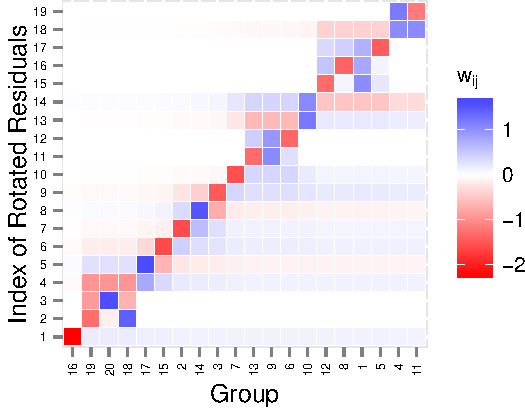
\includegraphics[width=0.4\textwidth]{cropped_cartoon_heatmap_raw.pdf}
	}
	\qquad
	\subfloat[$\bm{Q}\trans\bm{W}^{*\prime}$]{
		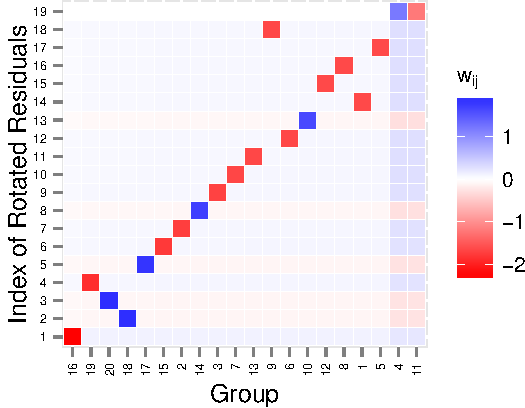
\includegraphics[width=0.4\textwidth]{cropped_cartoon_heatmap_varimax.pdf}
	}
	\caption{\label{fig:cartoon} Heat map of $\bm{W}^{*\prime}$ and $\bm{Q}\trans\bm{W}^{*\prime}$ for a simulated random intercept model with 20 groups. Applying the raw varimax rotation, $\bm{Q}$, reduces the number of groups loading on a given rotated residual.}
\end{figure}

\paragraph{Extension to multiple random effects.}
Up to this point our discussion has ignored that a model may (and often will) contain numerous random effects. In this case, the assumptions made on each random effect should be checked; thus, we propose assessing each random effect separately. To this end we must define linear combinations $\bm{L}_k$ such that $\bm{L}_k\trans \widehat{\bm{b}}$ produces the $k$th marginal random effect. For example, in a model with a random intercept and random slope, if $\bm{Z}$ is organized as a block diagonal matrix---that is $\bm{Z} = \bigoplus_{i=1}^{m} \bm{Z}_{i}$ where $\bigoplus$ denotes the direct sum \citep[page 47]{Gentle:2007}---then $\bm{L}_0 = \bm{I}_{m} \bigotimes ( 1,\ 0)$ produces the random intercepts and $\bm{L}_1 = \bm{I}_{m} \bigotimes ( 0,\ 1)$ produces the random slopes. The methodology presented in this section can be generalized to models with numerous random effects by substituting $\bm{L}_k\trans \widehat{\bm{b}}$ for $\widehat{\bm{b}}$.



%\aside{XXX I have started to restructure this subsection above, but will keep the original text below until I am done.}
%
%To combat  confounding between different  levels of residuals, we derive a reduced set of rotated residuals that are standardized, uncorrelated, and homoscedastic. We focus our discussion (and notation) on a two-level model with a single random effect in this section for ease of explanation, and describe how to extend this method at the end of this section.
%
%
%First, we define the \emph{fraction of confounding} for the random effects, which is minimized in the result below. This definition generalizes the fraction of confounding proposed by \cite{HildenMinton:1995wh}. 
%
%
%%\begin{definition}[Fraction of confounding]\label{def:fc1}
%%For the $i$th element of the target residual vector, $\widehat{\bm{e}}$, the fraction of confounding is given by
%%%
%%\begin{equation}\label{eq:fc}
%%	\text{FC}(\widehat{\bm{e}}_i) 
%%	= \frac{\bm{v_i}\trans \var(\widehat{\bm{e}} | \bm{e}) \bm{v_i}}
%%		{\bm{v_i}\trans \var(\widehat{\bm{e}}) \bm{v_i}}
%%	= \frac{\bm{v_i}\trans \bm{A} \bm{v_i}}
%%		{\bm{v_i}\trans \bm{B} \bm{v_i}}
%%\end{equation}
%%
%%where $\bm{v_i}$ is the $i$th column of the identity matrix.
%%%\todo[inline]{write this as a minimization problem}
%%%This rotation is given by $\bm{M} = \bm{T_r \Lambda_r}^{-1/2} \bm{U}$ where $\bm{T_r \Lambda_r}^{-1/2}$ is the inverse square root of $\bm{B}$ found through the spectral decomposition of $\bm{B}$ and $\bm{U}$ are the eigenvectors of $(\bm{\Lambda_r}^{-1/2} \bm{T_r}\trans) \bm{A} (\bm{\Lambda_r}^{-1/2} \bm{T_r}\trans)\trans$.
%%\end{definition}
%
%%Definition~\ref{def:fc1} describes the confounding for each element in the target residual vector individually. An overall measure of the amount of confounding is given below.\\
%
%%\begin{definition}\label{defc:fc2}
%%For the target residual vector, $\widehat{\bm{e}}$, the fraction of confounding is given by
%%%
%%\begin{equation}\label{eq:fc2}
%%FC(\widehat{\bm{e}}) = \mathrm{tr}( \var(\widehat{\bm{e}} | \bm{e} ) ) / \mathrm{tr}( \var(\widehat{\bm{e}}) ).
%%\end{equation}
%%\end{definition}
%
%%\begin{definition}[Fraction of confounding] \hh{define $\bm{b}$ and $\widehat{\bm{b}}$ as well}
%%Let $\bm{A} = \var(\widehat{\bm{b}} | \bm{b} )$ and $\bm{B} = \var(\widehat{\bm{b}})$, %which are positive semidefinite matrices by definition. \hh{that doesn't belong in a definition.}
%%\al{Also, let $\bm{W}$ be a linear transformation from the original $q$-dimensional space to an $s$-dimensional space ($s \leq q$).} \hh{Where does q come from? } The fraction of confounding in $\widehat{\bm{b}}$ \al{in this $s$-dimensional space} is given by
%%%
%%\begin{equation}\label{eq:fc2}
%%\text{FC}(s; \widehat{\bm{b}}) = \frac{1}{q} \tr\left( \left(\bm{W\trans B W} \right)\ginv \left(\bm{W\trans A W}\right) \right)
%%%\dfrac{1}{\ell} \displaystyle{\sum_i} \frac{\bm{v_i}\trans \bm{A} \bm{v_i}}
%%%		{\bm{v_i}\trans \bm{B} \bm{v_i}}.
%%\end{equation}
%%\hh{If FC only depends on s, you imply that for different Ws that have the same rank, you get the same FC. that's not true - so FC needs to be dependent on W. }
%%%where $\ell$ is the length of vector $\widehat{\bm{b}}$.
%%\end{definition}
%
%
%\begin{definition}[Fraction of confounding] 
%Let $\bm{b}$ denote a vector of $q$ random effects and $\widehat{\bm{b}}$ its predictions as defined in \eqref{eq:resid2}. For a full rank matrix $\bm{W} \in \mathbb{R}^{q \times s}$, where $ s \le q$, the fraction of confounding in the $s$-dimensional space spanned by $\bm{W}$ is defined as 
%\begin{equation}\label{eq:fc2}
%\text{FC}(\bm{W}; \widehat{\bm{b}}) = \frac{1}{q} \tr\left( \left(\bm{W\trans B W} \right)\ginv \left(\bm{W\trans A W}\right) \right),
%%\dfrac{1}{\ell} \displaystyle{\sum_i} \frac{\bm{v_i}\trans \bm{A} \bm{v_i}}
%%		{\bm{v_i}\trans \bm{B} \bm{v_i}}.
%\end{equation}
%where $\bm{B}$ is the covariance structure of $\bm b$, $\bm{B} = \var(\widehat{\bm{b}})$, and $\bm{A}$ is the conditional covariance structure of  $\widehat{\bm{b}}$ given $\bm{b}$,  i.e. $\bm{A} = \var(\widehat{\bm{b}} | \bm{b} )$.
%\end{definition}
%\noindent
%Note that both $\bm{A}$ and $\bm{B}$ are  positive semidefinite matrices by definition. 
%
%
%The fraction of confounding measures the contribution of the error terms  to the variance of the random effects. $\text{FC} \in [0,1]$, where 1 indicates that, due to confounding, the predicted random effects contain no information in addition to that found in the error terms, while 0 indicates no confounding. Notice that if $\bm{W}$ is the identity, then \eqref{eq:fc2} measures the fraction of confounding in the original vector of predicted random effects.
%
%
%In order to correct residuals for the impact of confounding, we propose using the linear transformation of the predicted random effects that substantially reduces the amount of confounding. To do this, we must determine the $s$-dimensional space in which confounding is substantially reduced and find the $\bm{W}$ that minimizes confounding within that space. To determine the dimension of the subspace spanned by the rotated residuals we propose the use of a  visual tool similar to the scree plots used for selecting the number of principal components. The construction of such plots depends on the linear transformation $\bm W$, so we first discuss the selection of $\bm{W}$ given  a fixed dimension $s$.
%
%\paragraph{Selecting the optimal linear transformation.}
%For a given $s$-dimensional space, the linear combination $\bm{W} \in \mathbb{R}^{q \times s}$ that minimizes \eqref{eq:fc2} also minimizes
%%
%\begin{equation}\label{eq:minimize}
%J_1(s) = \tr\left( \left(\bm{W\trans B W} \right)\inv \left(\bm{W\trans A W}\right) \right)
%%\displaystyle{\sum_i} \frac{\bm{v_i}\trans \bm{W} \bm{A} \bm{W}\trans \bm{v_i}}
%%		{\bm{v_i}\trans \bm{W} \bm{B} \bm{W}\trans \bm{v_i}}
%\end{equation}
%%
%Mathematically, this problem is solved using the generalized eigenvalue decomposition
%%
%\begin{equation}\label{eq:geigen}
%	\bm{Aw}_k = \gamma_k \bm{Bw}_k
%\end{equation}
%%
%where $\gamma_k$ and $\bm{w}_k$ are the $k$-th smallest eigenvalues and eigenvectors, respectively \citep{Fukunaga:1990}. 
%%thus, $\bm{W}^*$ consists of the eigenvectors associated with the $s$ smallest eigenvalues. 
%Computationally, we solve this problem by simultaneous diagonalization of $\bm{A}$ and $\bm{B}$ \citep{McDonald:1979ca, deLeeuw:1982to}. Simultaneous diagonalization of $\bm{A}$ and $\bm{B}$ requires $\bm{W}$ to be $\bm{B}$-orthogonal, so the optimal $\bm{W}$ is found to be
%%
%\begin{equation}\label{eq:optimw}
%	\bm{W}^*(s) = \argmin_{ 
%%\begin{scriptsize}
%%	\begin{cases}
%      \bm{W} \in \mathbb{R}^{q \times s}, \ \ 
%      \bm{W\trans B W} = \bm{I}
%%	\end{cases}
%%\end{scriptsize}
%	} 
%\tr\left( \bm{W\trans A W} \right) 
%\end{equation}
%%
%Below, we outline the procedure used to simultaneously diagonalize $\bm{A}$ and $\bm{B}$ for reference.\\
%%and refer the reader to \cite{McDonald:1979ca} and \cite{deLeeuw:1982to} for additional details on simultaneous diagonalization of two positive semidefinite matrices.\\
%
%\begin{algorithm}[Simultaneous diagonalization]
%Let $\bm{A}$ and $\bm{B}$ be two positive semidefinite matrices. The transformation that simultaneously diagonalizes both matrices can be found through the following procedure:
%\begin{enumerate}
%\item Find a transformation that whitens $\bm{B}$. Such a transformation is given by $\bm{T_r \Lambda_r}^{-1/2}$, where $\bm{T}_r$ and $\bm{\Lambda}_r$ are the first $r$  eigenvectors and eigenvalues of $\bm{B}$, where $r = \rank(\bm{B})$. 
%
%\item Transform $\bm{A}$ and $\bm{B}$ to
%\begin{align}
%\bm{\Lambda_r}^{-1/2} \bm{T_r}\trans \bm{A T_r \Lambda_r}^{-1/2} &= \bm{A}^* \label{eq:astar} \\
%\bm{\Lambda_r}^{-1/2} \bm{T_r}\trans \bm{B T_r \Lambda_r}^{-1/2} &= \bm{I}
%\end{align}
%
%\item Find an orthonormal transformation that diagonalizes $\bm{A}^*$. Such a transformation is given by the eigenvectors of $\bm{A}^*$, which we denote $\bm{U}$.
%\end{enumerate}
%
%\noindent
%Based on the above three steps, the transformation that simultaneously diagonalizes $\bm{A}$ and $\bm{B}$ is $\bm{T_r \Lambda_r}^{-1/2} \bm{U}$.\\ 
%\end{algorithm}
%
%The above procedure can be used to find the general solution to \eqref{eq:geigen}. To find the more specific transformation defined by \eqref{eq:optimw}, we focus on the $s$ eigenvectors associated with $s$ the smallest eigenvalues of $\bm{A}^*$, $\bm{U}_s$, making
%%
%\begin{equation}\label{eq:w}
%\bm{W}^* = \bm{T_r \Lambda_r}^{-1/2} \bm{U}_s
%\end{equation}
%%
%The rotated random effects are then given by $\bm{W}^{*\prime} \widehat{\bm{b}}$, which are standardized, uncorrelated, and homoscedastic (see the appendix for a proof).
%
%%\todo[inline]{Address that the order of the data will influence the resulting residuals.}
%%Since $\bm{B}$ is only positive semidefinite, it is important to note that the order of the groups in the data change the resulting residuals. In this case, the transformation in \eqref{eq:astar} eliminates a group
%
%
%%Having considered the computational aspects of the problem we must next consider the more practical aspects. 
%
%%\al{Having considered the optimal linear transformation for a given $s$-dimensional subspace, we return to the problem of selecting the dimension which substantially reduces the fraction of confounding.}
%
%
%\paragraph{Selecting the dimension of the subspace.}
%Selection of the dimension of the subspace spanned by the rotated residuals is central to our proposed method. Ideally, we would select the dimension such that the fraction of confounding is reduced to zero; however, this is not realistic in practice. Alternatively, we propose choosing the dimension that provides a substantial reduction in the fraction of confounding. Since our ultimate objective is distributional assessment, we must balance this reduction in the fraction of confounding with the loss in power of a test of the empirical distribution function (e.g., the Anderson-Darling test for normality) associated with dimension reduction. To guide this choice we suggest plotting the reduction in the fraction of confounding against the reduction in dimension, which is similar to the scree plot used to select the number of principal components. To illustrate the use of this plot we simulate two simple random intercept models with a group-level predictor:   model $M1$ has 40 groups of 30 observations and 10 groups of 5 observations;   model $M2$ also has 50 groups, with group sizes determined as random draws from either a Poisson(30) distribution (40 groups) or a Poisson(5) distribution (10 groups). %\todo[inline]{These two models are very similar. Go to a more extreme in the second model?}
% Figure~\ref{fig:elbow} shows two examples of such plots constructed for the simulated models. For both models, there is no decrease in the fraction of confounding for a one-dimensional reduction because a {one-dimensional reduction} simply adjusts for that rank deficiency of the covariance matrix, which can be thought of in terms of adjusting for the effective degrees of freedom. Both figures have an ``elbow'' in the plot corresponding to a reduction in the dimension of the subspace of 11; thus we would choose $s = 39$. { Additionally, we see that the elbow in the plot for model $M2$ is less pronounced. This occurs because the groups sizes are more unbalanced so the difference between the large and small group sizes is reduced.}
% 
%% \al{Talk about the differences here and why I chose these examples. Also talk about the loss of 1 d.f. More discussion here.}
%%
%\begin{figure}[htb]
%	\centering
%	 \subfloat[Model $M1$]{
%		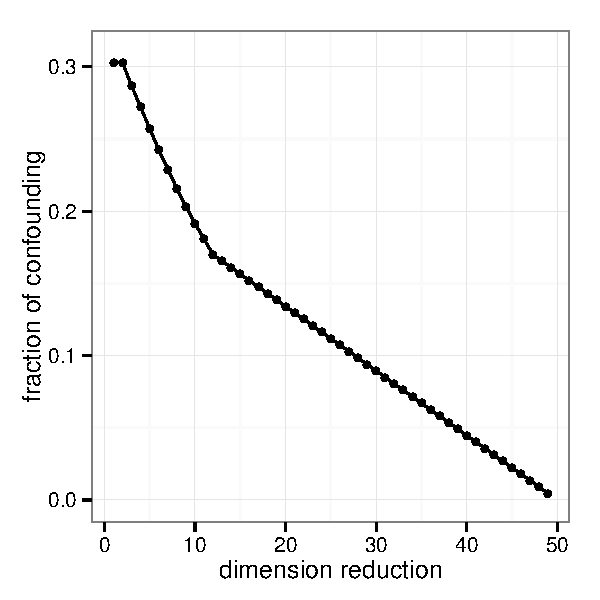
\includegraphics[width=0.4\linewidth]{elbow1.pdf}
%		}
%	  \subfloat[Model $M2$]{
%		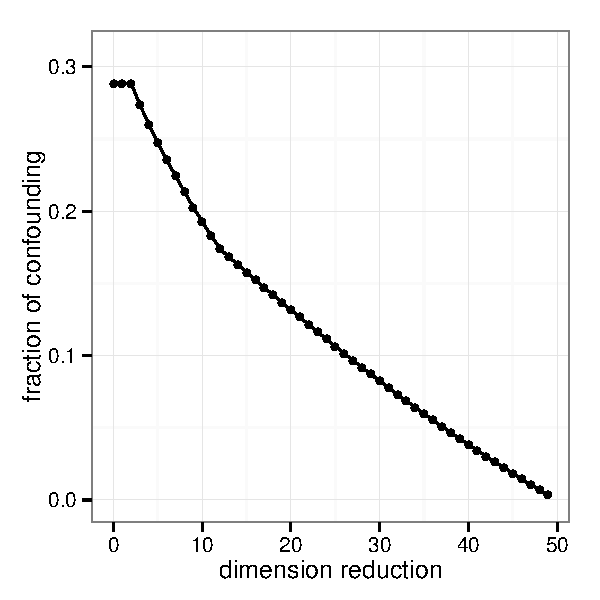
\includegraphics[width=0.4\linewidth]{elbow2.pdf}
%		}	
%	\caption{\label{fig:elbow} Plots of the fraction of confounding for each reduction in the dimension of subspace spanned by the rotated random intercepts from two simulation models. Model $M1$ has 50 groups: 40 groups of size 30, and 10 groups of size 5. Model $M2$ has 50 groups with group sizes determined as random draws from either a Poisson(30) distribution (40 groups) or a Poisson(5) distribution (10 groups). Based on these plots we  choose $s = 39$, corresponding to a dimension reduction of 11.}
%\end{figure}
%
%
%%%First, we must consider the selection of the dimension of the subspace spanned by the rotated residuals, $s$---that is, the length of the resulting transformed residual vector. 
%%For the level-1 residuals \cite{HildenMinton:1995wh} suggests using $s = \rank(\bm{B})$;
%%%One choice is $s = \rank(\bm{B})$, which aligns with the suggestion given by \cite{HildenMinton:1995wh} for the level-1 residuals. 
%%%This selection has the advantage that it works in all situations, but the disadvantage that the fraction of confounding will \al{often} not be \al{significantly} reduced. 
%%An alternative approach is to select $s$ based on the desired reduction in the fraction of confounding. \hh{You need to sell this point a bit more - what is the theoretical advantage of going down on the number of residuals? -- if the approach is to get FC down as much as possible, but have s at least 30, it is always going to end up at 30. What I still don't understand is that the minimization is not taking care of the percent of confounding to a higher degree, because that's really what it was supposed to do. }
%%%A starting point for this approach can be determined for a given reduction in the fraction of confounding by considering the relative contributions of the ordered diagonal elements of $\bm{B}\ginv\bm{A}$ to \eqref{eq:fc2}. 
%%We consider this approach in the simulation study presented in Section~\ref{sec:simulation} and present the results in Figure~\ref{fig:fc}. Note that in some situations it will not be possible to reduce the fraction of confounding much as the number of groups limits this reduction.
%
%\paragraph{Correcting for supernormality.}
%The transformation of the random effects results in a vector where each component is a linear combination of elements of $\widehat{\bm{b}}$. Consequently, the rotated residuals will appear more normal than the underlying distribution, if the underlying distribution is not normal. This issue is often referred to as supernormality \citep{Atkinson:1985}. One approach to address supernormality in this context is to reduce the number of elements in the linear combinations, which should reduce the extent of the problem. To do this, we suggest using an orthogonal rotation of $\bm{W}^*$, which we denote $\bm{Q}$, just as we rotate the factor loadings in factor analysis. Using this approach, the rotated residuals are obtained by $\bm{Q}\trans \bm{W}^{*\prime} \widehat{\bm{b}}$. One rotation that will produce rotated residuals comprised of a small number of raw residuals is the raw varimax rotation \citep{Johnson:2007}. Figure~\ref{fig:cartoon} displays heat maps of $\bm{W}^{*\prime}$ (left) and $\bm{Q}\trans\bm{W}^{*\prime}$ (right) for a simulated random intercept model with 20 groups, and demonstrates that the raw varimax rotation reduces the number of groups loading highly on each rotated residual. %\hh{what amount of confounding is there on the left and then on the right?} \al{The amount of confounding is the same between the right and the left. The only different between the two is that we applied the varimax transform to the plot on the right. Regardless, $FC \approx .25$. I used this small simulated model because I thought it showed what the varimax can do for us.} 
%Other orthogonal rotations could be used, but the varimax rotation is familiar to a wide range of analysts and is widely implemented in statistical software packages. A similar approach was used by \cite{Jensen:1999iu}, who used the raw varimax rotation to produce recovered errors for distributional assessment in the ordinary regression model.
%
%\begin{figure}[t]
%	\centering
%	\subfloat[$\bm{W}^{*\prime}$]{
%		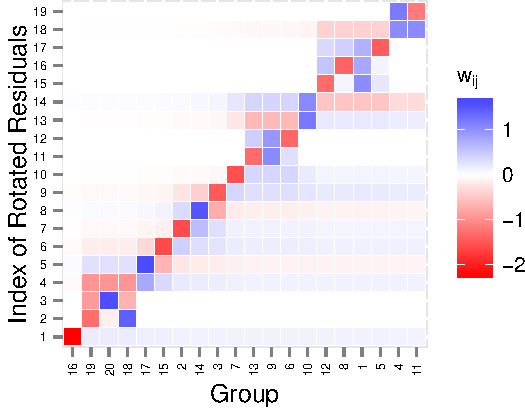
\includegraphics[width=0.4\textwidth]{cropped_cartoon_heatmap_raw.pdf}
%	}
%	\qquad
%	\subfloat[$\bm{Q}\trans\bm{W}^{*\prime}$]{
%		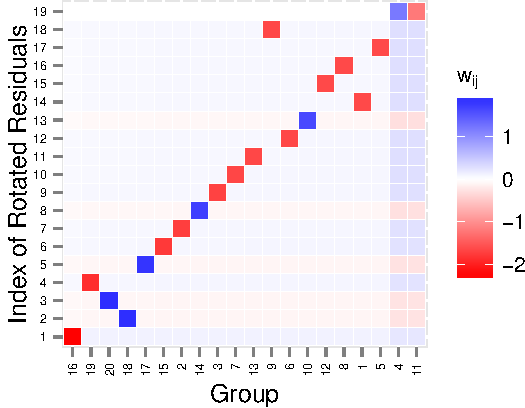
\includegraphics[width=0.4\textwidth]{cropped_cartoon_heatmap_varimax.pdf}
%	}
%	\caption{\label{fig:cartoon} Heat map of $\bm{W}^{*\prime}$ and $\bm{Q}\trans\bm{W}^{*\prime}$ for a simulated random intercept model with 20 groups. Applying the raw varimax rotation, $\bm{Q}$, reduces the number of groups loading on a given rotated residual.}
%\end{figure}
%
%\paragraph{Extension to multiple random effects.}
%Up to this point our discussion has ignored that a model may (and often will) contain numerous random effects. In this case, the assumptions made on each random effect should be checked; thus, we propose assessing each random effect separately. To this end we must define linear combinations $\bm{L}_k$ such that $\bm{L}_k\trans \widehat{\bm{b}}$ produces the $k$th marginal random effect. For example, in a model with a random intercept and random slope, if $\bm{Z}$ is organized as a block diagonal matrix---that is $\bm{Z} = \bigoplus_{i=1}^{m} \bm{Z}_{i}$ where $\bigoplus$ denotes the direct sum \citep[page 47]{Gentle:2007}---then $\bm{L}_0 = \bm{I}_{m} \bigotimes ( 1,\ 0)$ produces the random intercepts and $\bm{L}_1 = \bm{I}_{m} \bigotimes ( 0,\ 1)$ produces the random slopes. The methodology presented in this section can be generalized to models with numerous random effects by substituting $\bm{L}_k\trans \widehat{\bm{b}}$ for $\widehat{\bm{b}}$.


%----------------------------------------------------------------------------------
\section{Simulation study}\label{sec:simulation}
%----------------------------------------------------------------------------------

We conducted a simulation study to assess the specificity and sensitivity of tests of normality based on the two rotated residuals proposed in the previous section. 

\subsection{Design}\label{sec:sim-design}
%----------------------------------------------------------------------------------

%We examined situations in which we correctly and incorrectly reject the null hypothesis of normality---that is, power and type I error, respectively. We compute the percentage of Anderson-Darling (AD), Cram{\'e}r von Mises (CVM), and Kolmogorov-Smirnov (KS) tests that rejected the null hypothesis of normality.
% \hh{I think we don't need this sentence anymore - it should be clear from the discussion in the beginning} These test statistics each measure the discrepancy between the empirical distribution of the rotated random effects and assumed distribution of the random effects \al{XXX think carefully about this sentence...}, which sheds light on the behavior of Q-Q plots constructed from the rotated residuals. 


The design matrices from model \eqref{eq:radon} were used as templates for realistic data generation;  for simplicity of the simulation design, only the 60 counties with full rank $\bm{Z}$ matrices were included. 
Normal, heavy-tailed, and skewed distributions were used to generate the simulated errors and random effects. We used a rescaled $t$ distribution with 3 degrees of freedom to generate heavy tailed residuals, and a centered and rescaled exponential distribution with a rate parameter of 1 to generate skewed residuals. For simplicity we required the distributions of the random slope and intercept to the be same and assumed independence between the random effects. The nine distributional settings considered in the simulation study are summarized in Table~\ref{tab:simdsns}.
%
\begin{table}[htdp]
\centering
\caption{\label{tab:simdsns} A summary of the nine distributional settings considered in the simulation study.}
\begin{tabular}{llccc}\hline
Distributions of & & \multicolumn{3}{c}{Random effects, $F_2$} \\ \cline{3-5}
           & & $\mathcal{N}(0, \ \sigma^2_{b})$ & $(\sigma_{b} / \sqrt{3})\, t_3$ & $\sigma_{b} \, \{ \text{Exp}(1) - 1 \}$ \\ \hline
Error terms, $F_1$  & $\mathcal{N}(0, \ \sigma^2_{\varepsilon})$       & &&\\
             & $(\sigma_{\varepsilon} / \sqrt{3})\, t_3$  &  & $\varepsilon_{ij}^* \overset{iid}{\sim} F_1, \ \ b_{0i}^*, b_{1i}^* \overset{iid}{\sim} F_2$ &  \\
             & $\sigma_{\varepsilon} \, \{ \text{Exp}(1) - 1 \}$       & && \\ 
\hline
\end{tabular} 
\end{table}
%
The fixed effects coefficients were set to the maximum likelihood estimates.

To investigate the effect that pooling has on the rotated random effects we considered  three variance structures to represent different degrees of confounding for the random effects:\\
%
\begin{tabular}{ll}
\textbf{high:} & $\sigma^2_\varepsilon = 4$ and  $\sigma^2_{b_0} = \sigma^2_{b_1} = 1$ \\
\textbf{moderate:} & $\sigma^2_\varepsilon = 1$ and  $\sigma^2_{b_0} = \sigma^2_{b_1} = 1$ \\
\textbf{low:} & $\sigma^2_\varepsilon = 1$ and  $\sigma^2_{b_0} = \sigma^2_{b_1} = 4$ \\
\end{tabular}
%

Under each simulation setting 1000 data sets were generated for each model and the rotated residuals were obtained using $s = \rank(\bm{B})$ (which is 58 and 59 for the random intercept and slope, respectively) as well as $s =$ 55, 50, 45, 40, 35, and 30.  The percentage of AD, CVM, and KS tests that rejected the null hypothesis of normality were recorded.

We ran the above simulation both in the case where $\bm{D}$ and $\bm{R}$ were known and where $\bm{D}$ and $\bm{R}$ were estimated. The results were quite similar between these two simulation studies, so we present the results from the simulation study for estimated  $\bm{D}$ and $\bm{R}$, as this reflects more closely what is done in practice. Full simulation results are available in the supplement.


\subsection{Results}\label{sec:sim-results}
%----------------------------------------------------------------------------------
\noindent
Figure~\ref{fig:fc} shows the average fraction of confounding for the rotated random intercept (left) and random slope (right) over the different values for $s$ for each variance structure. As $s$ is reduced, the fraction of confounding is reduced, which aligns with the expectation that smaller choices of $s$ reduce the contributions of more highly confounded groups.

\begin{figure}[h]
	\centering
	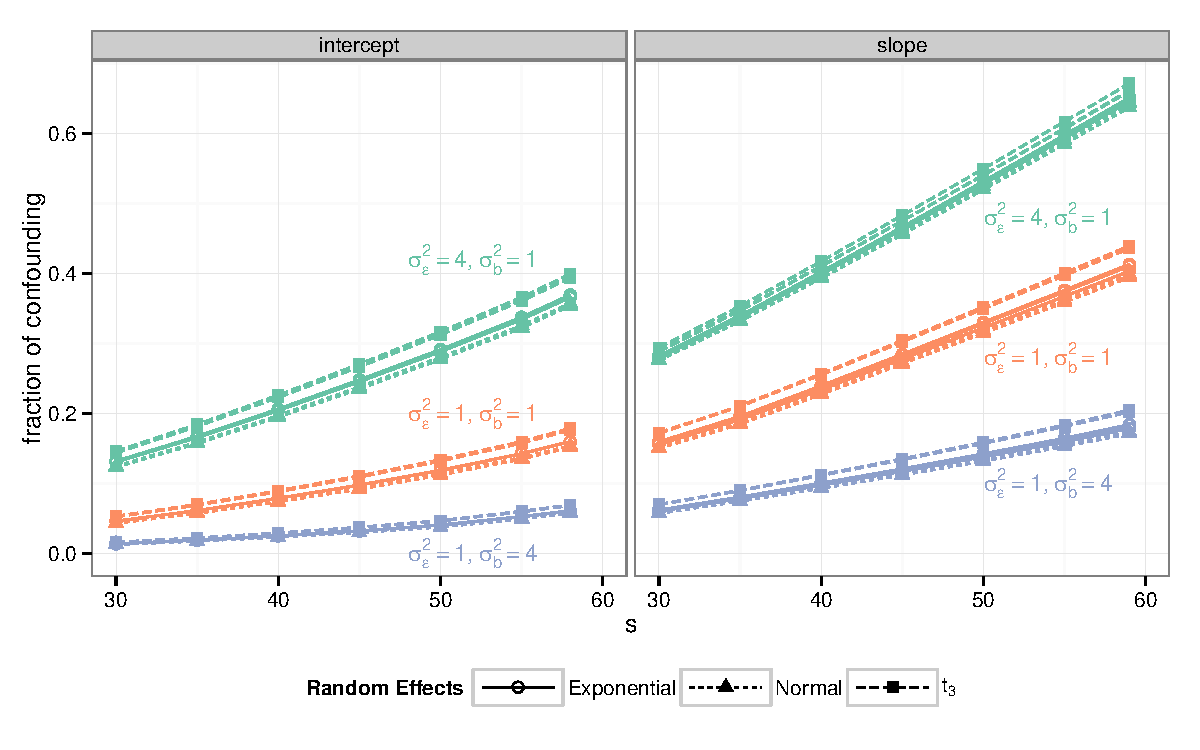
\includegraphics[width=0.9\textwidth]{fc_by_s.pdf}
	\caption{\label{fig:fc} Change in the fraction of confounding (FC) as the dimension of the rotated random effects vector, $s$, is reduced for the three variance structures considered in the simulation study. %LOESS smoothers estimate the trajectory of FC as $s$ varies.} 
	}
\end{figure}

Table~\ref{tab:results-int} and Figure~\ref{fig:results-slope} display the estimated type I error rates using the AD normality test ($\alpha = 0.05$) on the rotated and varimax rotated random intercepts and random slopes, respectively, when $\sigma^2_\varepsilon = 4$ and $\sigma^2_{b_0} = \sigma^2_{b_1} = 1$. The CVM and KS tests performed similarly and are omitted for brevity (full simulation results can be found in the supplementary material). Both figures show that the type I error rate is stabilized close to the nominal level with the appropriate choice of $s$. For the random intercept most choices of $s$ perform reasonably well, with the type I error rate closest to the nominal level for all error distributions between 30 and 40. For the random slope, $s$ must be chosen to be 30 for type I error to be near the nominal level; however, $s$ may need to be even smaller to achieve the nominal rate. 


\begin{figure}[h]
	\centering
	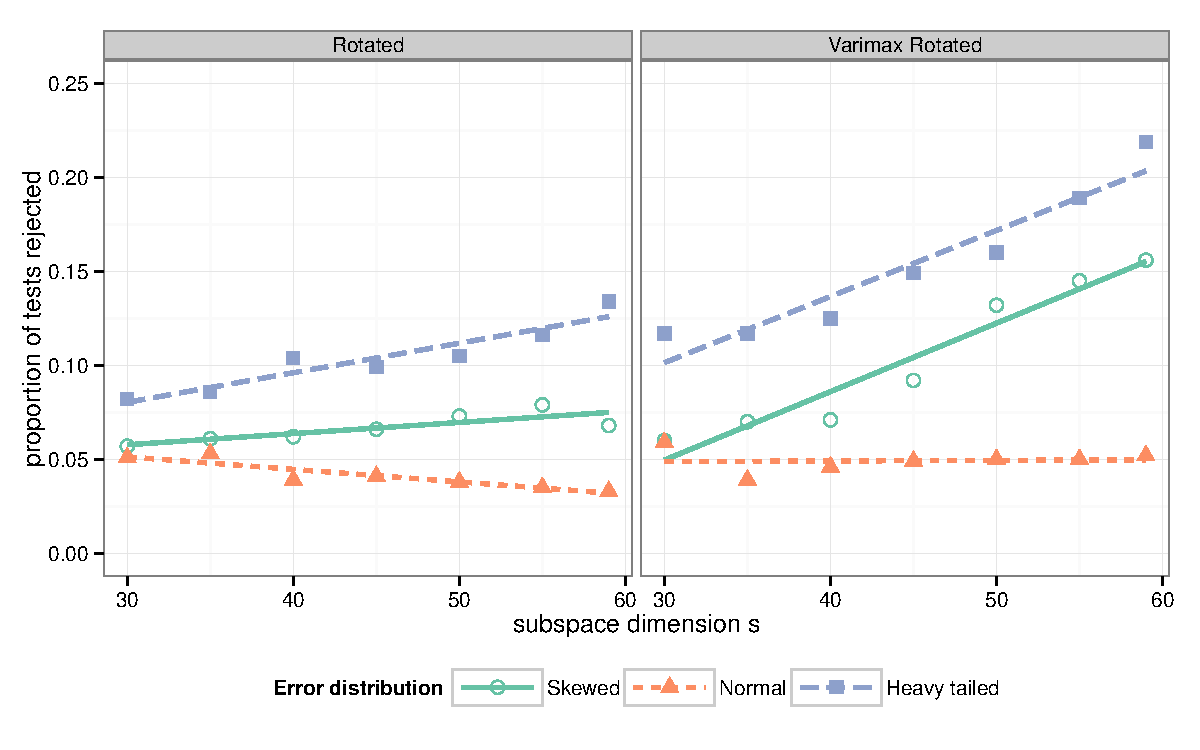
\includegraphics[width=0.9\textwidth]{ad_slope_results.pdf}
	\caption{\label{fig:results-slope} Estimated type I error rate using the Anderson-Darling normality test ($\alpha = 0.05$) on the rotated random slopes (left) and varimax rotated random slopes (right) by the distribution of the error terms and $s$.}
\end{figure}

Table~\ref{tab:results-int} and Figure~\ref{fig:power-slope} show the estimated power of the AD test ($\alpha = 0.05$) on the rotated and varimax rotated random intercepts and random slopes, respectively, for the highly confounded variance structure. The estimated power to detect non-normal random effects distributions is amplified by the varimax rotation and larger choices of $s$. We also find that the estimated power is lower than would be expected from randomly sampled values from an exponential or $t_3$ distribution (what we will refer to as the ``gold standard''). 
%\hh{the gold standard should show in your figures as well, so that we have a way of gauging the loss in power other than perfect power of 1, which is going to make any gain in power look small.} 
%\al{I can do this, but the power for detecting the exponential at these sample sizes is very high, which makes things look small. The AD test has less power to detect the t distribution at these sample sizes.}
For example, when $s=30$, simulations indicate the power of the AD test to detect a $t_3$ distribution to be approximately 0.4, whereas our simulations indicate nearly half the power, with the random slope generally having lower power than the random intercept. Interestingly,  there is higher power to detect a heavy tailed distribution than a skewed distribution.  Additional simulations (not shown) using a model with a continuous variable defining the random slope showed results similar to the random intercept (Table~\ref{tab:results-int}).


While the estimated power is lower than the gold standard, the fact that the type I error rate can be stabilized indicates that distributional problems detected using the rotated random effects will truly be problems; thus, providing more diagnostic information than the (unrotated) predicted random effects.


\begin{figure}
	\centering
	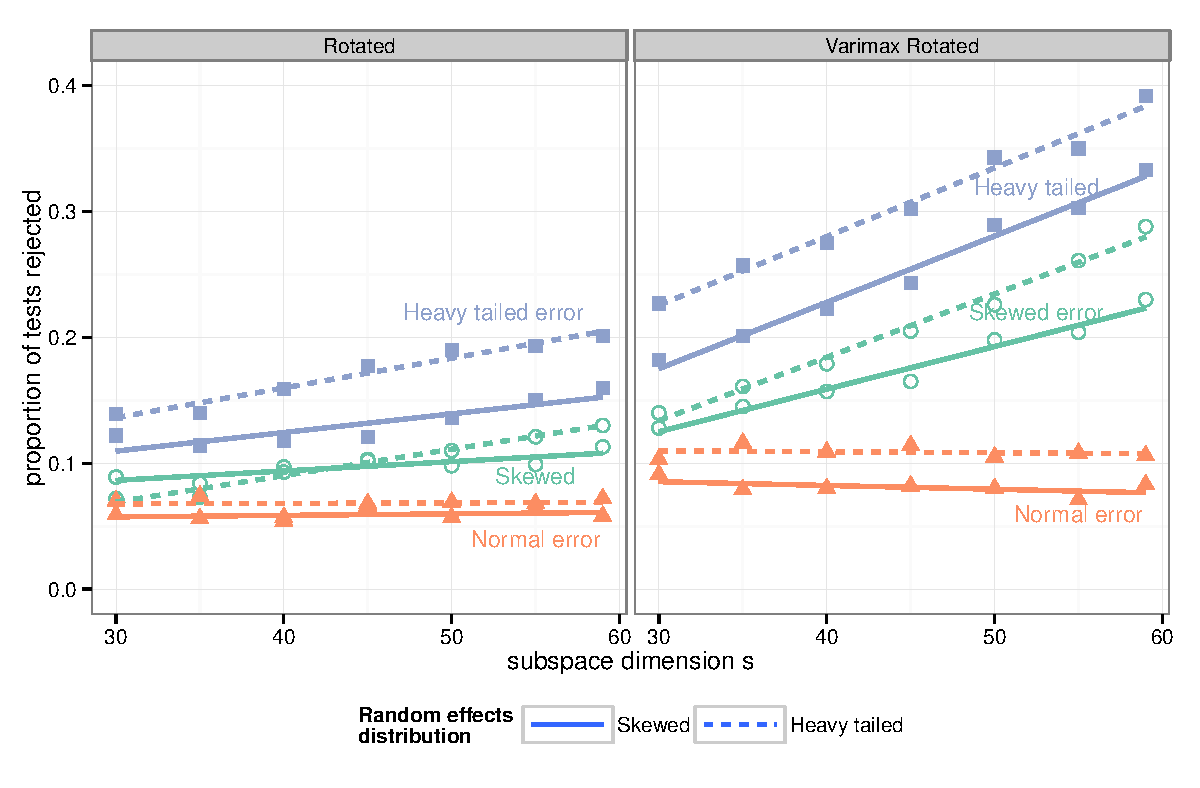
\includegraphics[width=0.9\textwidth]{ad_slope_power.pdf}
	\caption{\label{fig:power-slope}Linear smoother of the estimated power using the Anderson-Darling normality test ($\alpha = 0.05$) on the rotated random slopes (left) and varimax rotated random slopes (right) by $s$. The color denotes the distribution of the errors and the line type denotes the distribution of the random slope.}
\end{figure}


\begin{table}
\centering
\caption{\label{tab:results-int} Percentages of AD tests rejecting the null hypothesis of normality at the 5\% significance level for the rotated (a) and varimax rotated (b) random intercepts by $s$. The gray shading indicates the situations where the random intercept is normal (i.e., type I error).}
\subfloat[Rotated random intercept.]{
	\begin{tabular}{ll rrrrrrr} \hline
	& & \multicolumn{7}{c}{$s$} \\ \cline{3-9}
	Random intercept & Error term & 58 & 55 & 50 & 45 & 40 & 35 & 30\\ \hline 
\rowcolor{gray!20}Normal	&	Normal			& 4.4	& 	4.0	& 4.6	& 4.3	&	4.4	&	5.0	&	5.7 \\
\rowcolor{gray!20}	    &	Heavy tailed		& 7.5	&	7.6	& 6.7	& 6.2	&	5.0	&	4.2	&	5.0 \\	
\rowcolor{gray!20}	    &	Skewed			& 5.1	&	4.7	& 5.7	& 5.8	&	5.6	&	5.5	&	5.6 \\	
&&&&&&&&\\
Heavy tailed	&	Normal		& 13.9	&	13.6	& 13.1	& 13.4	&	13.0	&	13.1	&	12.1 \\	
	        & Heavy tailed	& 19.0	&	18.6	& 16.7	& 16.1	&	16.0	&	14.8	&	13.9 \\	
			& Skewed			& 15.5	&	15.1	& 14.2	& 13.6	&	13.2	&	12.7	&	11.9 \\
&&&&&&&&\\
Skewed	&	Normal			& 9.6	&	8.7	& 9.5	& 9.7	&	10.0	&	11.0	&	10.0 \\	
		&	Heavy tailed		& 12.6	&	12.5	& 12.0	& 11.3	&	10.1	&	11.3	&	11.0 \\	
		&	Skewed			& 13.4	&	13.4	& 12.2	& 12.2	&	11.0	&	11.3	&	10.8 \\
\hline
	\end{tabular}
}

\subfloat[Varimax rotated random intercept.]{
	\begin{tabular}{ll rrrrrrr} \hline
	& & \multicolumn{7}{c}{$s$} \\ \cline{3-9}
	Random intercept & Error term &  58 & 55 & 50 & 45 & 40 & 35 & 30\\ \hline
\rowcolor{gray!20}Normal	&	Normal			& 	4.9	& 	5.3	&	5.2	&	5.3	&	5.3	&	5.2	&	5.5	\\
\rowcolor{gray!20}	    &	Heavy tailed		& 	9.0	&	9.1	&	8.0	&	7.1	&	6.0	&	5.1	&	5.2	\\
\rowcolor{gray!20}	    &	Skewed			& 	5.2	&	5.1	&	4.4	&	5.5	&	6.1	&	5.1	&	6.1	\\
&&&&&&&&\\
Heavy tailed	&	Normal		& 	22.1	&	22.3	&	23.3	&	22.9	&	23.3	&	22.3	&	21.6	\\
	        & Heavy tailed	& 	34.4	&	33.3	&	32.1	&	31.6	&	30.1	&	27.0	&	26.6	\\
			& Skewed			& 	27.8	&	26.7	&	25.6	&	27.0	&	24.4	&	23.1	&	21.8	\\
&&&&&&&&\\
Skewed	&	Normal			& 	19.7	&	21.2	&	21.3	&	22.1	&	22.7	&	21.1	&	22.3	\\
		&	Heavy tailed		& 	29.7	&	28.4	&	27.1	&	25.0	&	25.5	&	25.0	&	23.8	\\
		&	Skewed			& 	22.2	&	23.5	&	21.7	&	23.1	&	21.1	&	22.9	&	21.1	\\
\hline
	\end{tabular}
}
\end{table}


%----------------------------------------------------------------------------------
\section{Radon data: Revisited}\label{sec:radon2}
%----------------------------------------------------------------------------------
%Next, we return to the motivating example and use rotated residuals to assess the distribution of the random effects using the rotated random effects. 
\noindent
Recall that in Section~\ref{sec:ex} we determined that the error terms were not normally distributed. Consequently, examination of Q-Q plots of the predicted random effects will likely lead to erroneous conclusions due to the high degree of shrinkage. 

In order to construct Q-Q plots of the rotated random effects we first consider the choice of $s$. For model \eqref{eq:radon} the high degree of shrinkage leads to a large fraction of confounding for each random term: 0.72 for the random intercept and 0.70 for the random slope. In choosing $s$ we wish to substantially reduce the fraction of confounding, but restrict attention to $s \geq 30$ so as not to decrease the maximum possible power of a normality test too severely. Figure~\ref{fig:radon-dim} shows the fraction confounding for $s \geq 30$. 
%
%\todo[inline]{We could show this in a plot if room isn't an issue. The below are just to show what the plots look like... There is really no elbow because of the sample sizes involved in the radon example, so I don't know if we want to discuss them again here. }
%\hh{It should be either the table or the graphic. I'd be fine with either, but it would strengthen the graphical component of the paper to have the plots here. } 

\begin{figure}
\centering
	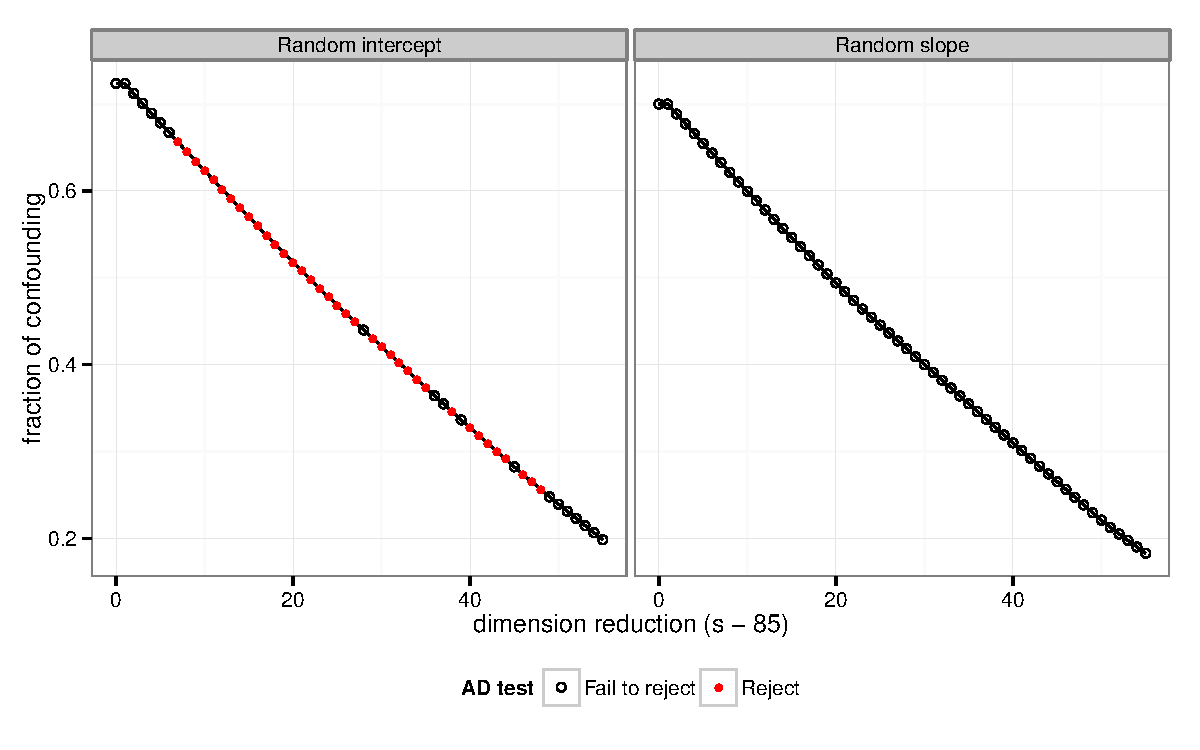
\includegraphics[width=0.9\textwidth]{radon_elbows.pdf}
	\caption{\label{fig:radon-dim} Plots of the fraction of confounding for each reduction in the dimension of subspace spanned by the rotated random intercept (left) and random slope (right) for the radon example. Filled points represent situations in which the AD test rejects normality of the varimax rotated random effects.}
\end{figure}


%\begin{table}[ht]
%\centering
%\caption{\label{tab:s} The fraction of confounding for the rotated random effects at various settings of $s$ for model \eqref{eq:radon}. \hh{At which dimension does the normality test switch from rejection to acceptance?} \al{This happens right away, rank(B), for the slope and around 40 for the intercept.}}
%\begin{tabular}{rrrrrrr}
%  \hline
%subspace dimension  $s$         & 30 & 40 & 50 & 60 & 70 & 80 \\ \hline
%  Intercept & 0.56 & 0.60 & 0.63 & 0.66 & 0.69 & 0.72 \\ 
%  Slope     & 0.52 & 0.56 & 0.60 & 0.63 & 0.66 & 0.70 \\ 
%   \hline
%\end{tabular}
%\end{table}
%
%\todo[inline]{This is a first attempt at the rework, I am still a little tongue tied here. I really like figure 10 and how it helps guide the decision and shows that the dimension is less critical, but that makes explaining the choice to show example Q-Q plots a bit blurry.}
We do not find elbows for either random effect in plots of the fraction of confounding against the reduction in dimensionality (Figure~\ref{fig:radon-dim}) making the choice of the dimension more difficult; however, because of the large number of counties with few observations, the smoothness of the plots is not unexpected. For a decision on the distribution, the exact choice of the subspace dimension $s$ is also not particularly critical. The color (fill) of the points in figure~\ref{fig:radon-dim} shows %As an additional aid to select the dimension, we considered 
the results of the AD test at the 5\% significance level for each dimension. The red (solid) points denote a rejection of the null hypothesis of normality. %Considering the results of the AD test, we find the choice exact choice of the dimension of the subspace to be less critical as 
The results are stable until the dimensionality is reduced to the point where  the AD test lacks power. To show an example of the Q-Q plots produced from the rotated random effects Figure~\ref{fig:rotate-radon} shows Q-Q plots of the rotated random effects for subspace $s = 65$. %, which results in approximately a 30\% reduction of the fraction of confounding. Figure~\ref{fig:rotate-radon} shows Q-Q plots of the marginal rotated random effects. 
We see that the random intercept significantly deviates from the assumption of normality while the random slope does not.


\begin{figure}[htb]
	\centering
	 \subfloat[Random intercept]{
		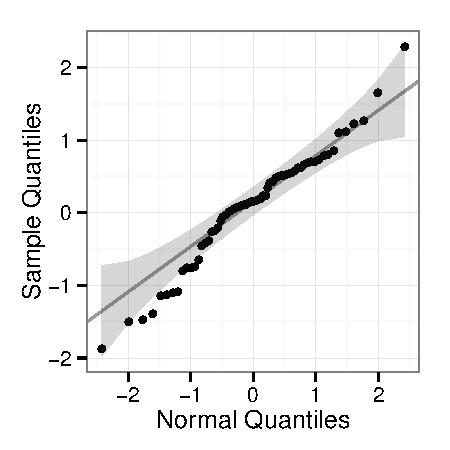
\includegraphics[width=0.35\linewidth]{rotatedQQ-intercept.pdf}
		}
	  \subfloat[Random slope]{
		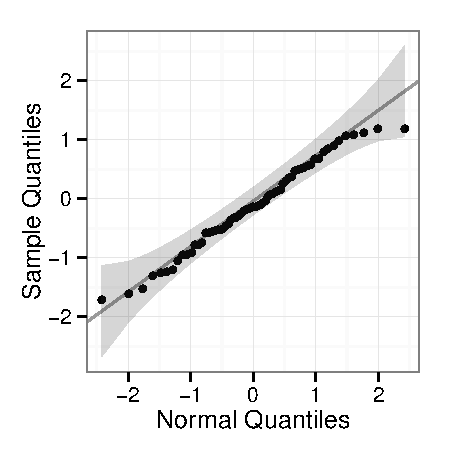
\includegraphics[width=0.35\linewidth]{rotatedQQ-slope.pdf}
		}	
	\caption{\label{fig:rotate-radon} Normal Q-Q plots with point-wise 95\% confidence bands of the marginals rotated random effects. The deviations from normality are much less pronounced than before, resulting in the failure to reject the null hypothesis of normality in the case of the random slope.} %\hh{what do the normality tests say?} \al{The tests all say fail to reject.}}
\end{figure}


%----------------------------------------------------------------------------------
\section{Discussion}\label{sec:discussion}
%----------------------------------------------------------------------------------

In this paper we have discussed two graphical approaches to assess the distributional assumptions made on the random effects in hierarchical linear models. The first approach used the lineup protocol to compare the predicted random effects produced in estimating the observed model to those produced when estimating a properly specified model. This method only assumes a distributional specification for the random effects and does not directly compare the predicted random effects to their distribution. Consequently, the conclusions that are drawn from this approach relate to evidence that the predicted random effects either are or are not {consistent} with what is expected under a correctly specified random effects distribution. The second approach rotates the predicted random effects so as to be able to compare them directly to the hypothesized distribution using a Q-Q plot. We have shown that the rotated random effects are standardized, uncorrelated, and homoscedastic, and that the rotation addresses the confounding present allowing for the random effects to be targeted separately from the error terms. 
% While the loss in power due to the rotation may be troubling, we found the lack of diagnostic information in the predicted random effects to be the bigger concern. \al{XX The last sentence might not be needed if we keep the last paragraph as it is.}

Under either approach, a misspecified covariance structure may lead to erroneous rejection of the null hypothesis. Therefore, in practice we recommend an assessment of the structure of {the within- and between-group covariance matrices} prior to distributional assessment.
%\todo[inline]{R and D have been introduced way back - rather than using the symbols, describe the matrices in words.}. 
An alternative approach would be the use of robust covariance estimation techniques to protect against such misspecification; however, {it is not clear how this impacts the diagnostic tools. We will leave this investigation for future study.} %we are unsure of its impact on these diagnostic tools, which is an are for future study.

It is important to note that formal tests have been proposed  to detect mixture distributions in the random effects \citep{Verbeke:1996va} and for overall goodness-of-fit tests for both the error terms and random effects \citep{Jiang:2001dx}; however, these methods do not lend themselves to graphical inspection and have not been implemented in statistical software. Our method, on the other hand, requires only byproducts of the model fitting procedure and the use of matrix decompositions for simultaneous diagonalization, which are widely accessible in standard software. All of the methods and graphics discussed in this paper are implemented in  \texttt{R} \citep{R}. In particular, the rotated residuals are part of the package \texttt{HLMdiag} \citep{HLMdiag, Loy:JSS}.
%Following from this result, the pointwise confidence bands shown were not unique to this method, but follow from the development of the normal Q-Q plot (FIND REFERENCE), and were provided as an aid to interpretation, not as a formal test.

%\todo[inline]{The paragraphs below here need to be reworked/rethought based on the rewritten paragraphs above.}

Simulation has revealed that tests of normality using the rotated random effects achieve approximately nominal type I error rates with appropriate choice of the dimension, $s$. This indicates that assessment of the rotated residuals can target the distribution of the random effects in the presence of pooling, which the predicted random effects cannot. The power to detect non-normal random effects distributions is lower than the gold standard, which is to be expected as the rotated residuals consist of sums of predicted random effects, resulting in a total distribution that is closer to a normal distribution than its individuals.  %we have taken linear combinations of predicted random effects in our rotation. 
The varimax rotation reduces the impact of this supernormality effect. %, but other orthogonal rotations (i.e., quartimax) may perform better resulting in increased power and is an area for future investigation. 
While we do think that the loss in power is troubling,
%We believe the loss of power is less troubling than
 the inflated type I error rates resulting from high levels of confounding is of a much bigger concern. Unlike before,  any detection of a distributional deviation can now be trusted even in situations with high amounts of  confounding between the levels of residuals.

  
%  This indicates that the predicted random effects do contain useful diagnostic information even when models are highly confounded, but not in their ``raw'' state.
 
%It is important to note that the procedure outlined in this paper assumes that the covariance structures in the hierarchical linear model are correctly specified. If this is not the case, then we would expect this model violation to affect assessment of the rotated random effect. Therefore, in practice we recommend an assessment of the covariance structures prior to distributional assessment. It would be of interest to assess the effectiveness of this methodology with robust covariance estimation techniques.

%\todo[inline]{Should I talk about the more alternative objective function that I have recently discovered that might lead to better results but is computationally more complex as there is no closed form solution? I see this as an area of future investigation, but I don't know how much of that is conventional to put in the article.}

%\todo[inline]{Things to return to in the discussion (moved from elsewhere)}
%\hh{the next paragraph needs a bit of attention. my first reaction as a reviewer would be to say - ok, it's not graphical, but how do those tests do? It distracts a bit from the main intention of the paper. I'd be in favor to remove the paragraph from here and maybe leave it for the discussion that there are other , non-graphical tests. }
%\al{I see your point. I will work on incorporating this to the discussion.}
%Several methods to assess the random effects distribution have been proposed. Formal tests have been proposed to to detect mixture distributions \citep{Verbeke:1996va} in the random effects and for overall goodness-of-fit tests for both the error terms and random effects \citep{Jiang:2001up}; however, these methods do \hh{not} lend themselves to graphical inspection and have not been implemented in statistical software.


% If a graphical assessment of the random effects distribution is not desired, then there are other available methods for model assessment \cite[c.f., the $\chi^2$ test proposed by][]{Jiang:2001up}, but they do not lend themselves to graphical inspection. While such goodness-of-fit tests can detect distributional deviations, they do not suggest how the assumption as been violated. 

%The rotated random effects can be used with Q-Q plots, which are familiar to analysts. 
%The use of the rotated random effects results in approximately nominal type I error rates when the dimension, $s$, is properly chosen; however, simulations have revealed that tests using the rotated random effects have low power to detect non-normal alternatives. Despite this fact, the rotated random effects present a method allowing for the predicted random effects to be used in distributional assessment, and when a deviation is detected one has cause to believe this detection, which previously not the case for highly confounded models. Additionally, this method is far less computationally demanding than simulation-based assessments, such as simulation envelopes for Q-Q plots, which are not guaranteed to work in situations with high levels of confounding (see the supplemental materials). Also, orthogonal rotations other than the varimax rotation (such as the quartimax rotation) may provide additional power, and is an area for future investigation. 



%\todo[inline]{
%Summarize everything and talk about future directions (if there are any). I have started a list below}
%\begin{itemize}
%\item Discuss the relative speed of this procedure to a bootstrap procedure
%\item Discuss why we are not using the ``upward'' residuals analysis approach discussed in the lit review chapter.
%\end{itemize}

%----------------------------------------------------------------------------------
\section{Acknowledgments}
%----------------------------------------------------------------------------------
The authors would like to thank the associate editor and reviewers whose comments and suggestions substantially improved the paper.

%----------------------------------------------------------------------------------
\section{Appendix: Additional technical details}
%----------------------------------------------------------------------------------

\subsection{Simultaneous diagonalization}

Below, we outline the procedure used to simultaneously diagonalize $\bm{A}$ and $\bm{B}$ for reference.
%and refer the reader to \cite{McDonald:1979ca} and \cite{deLeeuw:1982to} for additional details on simultaneous diagonalization of two positive semidefinite matrices.\\

\begin{algorithm}[Simultaneous diagonalization]
Let $\bm{A}$ and $\bm{B}$ be two positive semidefinite matrices such that the kernel of B is a subspace of the kernel of $\bm{A}$. The transformation that simultaneously diagonalizes both matrices can be found through the following procedure:
\begin{enumerate}
\item Find a transformation that whitens $\bm{B}$. Such a transformation is given by $\bm{T_r \Lambda_r}^{-1/2}$, where $\bm{T}_r$ and $\bm{\Lambda}_r$ are the first $r$  eigenvectors and eigenvalues of $\bm{B}$, where $r = \rank(\bm{B})$. 

\item Transform $\bm{A}$ and $\bm{B}$ to
\begin{align}
\bm{\Lambda_r}^{-1/2} \bm{T_r}\trans \bm{A T_r \Lambda_r}^{-1/2} &= \bm{A}^* \label{eq:astar} \\
\bm{\Lambda_r}^{-1/2} \bm{T_r}\trans \bm{B T_r \Lambda_r}^{-1/2} &= \bm{I}
\end{align}

\item Find an orthonormal transformation that diagonalizes $\bm{A}^*$. Such a transformation is given by the eigenvectors of $\bm{A}^*$, which we denote $\bm{U}$.
\end{enumerate}

\noindent
Based on the above three steps, the transformation that simultaneously diagonalizes $\bm{A}$ and $\bm{B}$ is $\bm{T_r \Lambda_r}^{-1/2} \bm{U}$.\\ 
\end{algorithm}


\subsection{Rotated random effects are standardized, uncorrelated, and homoscedastic}

We present the proof of the claim that the rotated residuals, $\bm{W}^{*\prime} \widehat{\bm{b}}$, are standardized, uncorrelated, and homoscedastic. Following the developments presented in Section~\ref{sec:rotate}, we present this discussion for the random effects assuming that there is only a random intercept. Generalization to the situation with multiple random effects follows as previously discussed.

\begin{proof}
 Let $\bm{A} = \var(\widehat{\bm{b}} | \bm{b})$, $\bm{B} = \var(\widehat{\bm{b}})$, $r = \text{rank}(\bm{B})$, and $q = $ the number of elements in $\widehat{\bm{b}}$. Recall that $\bm{A}$ and $\bm{B}$ are symmetric and positive semidefinite. Following from above, $\bm{T}_r$ and $\bm{\Lambda}_r$ follow from the spectral (or eigenvalue) decomposition of $\bm{B} = \bm{T_r \Lambda_r T_r}\trans$, and $\bm{U}$ follows from the spectral decomposition of $\bm{A^*} = \bm{\Lambda_r}^{-1/2} \bm{T_r}\trans \bm{A T_r \Lambda_r}^{-1/2} = \bm{U} \bm{\Gamma} \bm{U}\trans$. Then, 
\begin{align*}
\var(\bm{W}^{*\prime} \widehat{\bm{b}}) &= \var(\bm{U}\trans \bm{\Lambda_r}^{-1/2} \bm{T_r}\trans \widehat{\bm{b}})\\
&= (\bm{U}\trans \bm{\Lambda_r}^{-1/2} \bm{T_r}\trans) \var(\widehat{\bm{b}}) (\bm{T_r \Lambda_r}^{-1/2} \bm{U})\\
&= (\bm{U}\trans \bm{\Lambda_r}^{-1/2} \bm{T_r}\trans) \bm{B} (\bm{T_r \Lambda_r}^{-1/2} \bm{U})\\
&= \bm{I}
\end{align*}
proving that the rotated random effects are standardized, uncorrelated, and homoscedastic.
\end{proof}

\subsection{Lineup details}\label{sec:detrended}
As an alternative to the standard Q-Q plot, a detrended version of Q-Q plots (see figure~\ref{fig:lineup-2}) was shown to participants in a study. In the detrended Q-Q plot, the plot is rotated by 45$^\circ$ to make comparisons between the line of identity and the empirical distribution function a cognitively easier task. However, for assessing normality of the random effects distribution, the results from both types of plots were very similar. None of the participants identified the observed data as the most different panel from the set, while panel \#$(3^2+3)$ was the one picked by most participants. Table~\ref{tab:lpresults} gives an overview of the results from the study. 
\begin{figure}[htb]
	\centering
	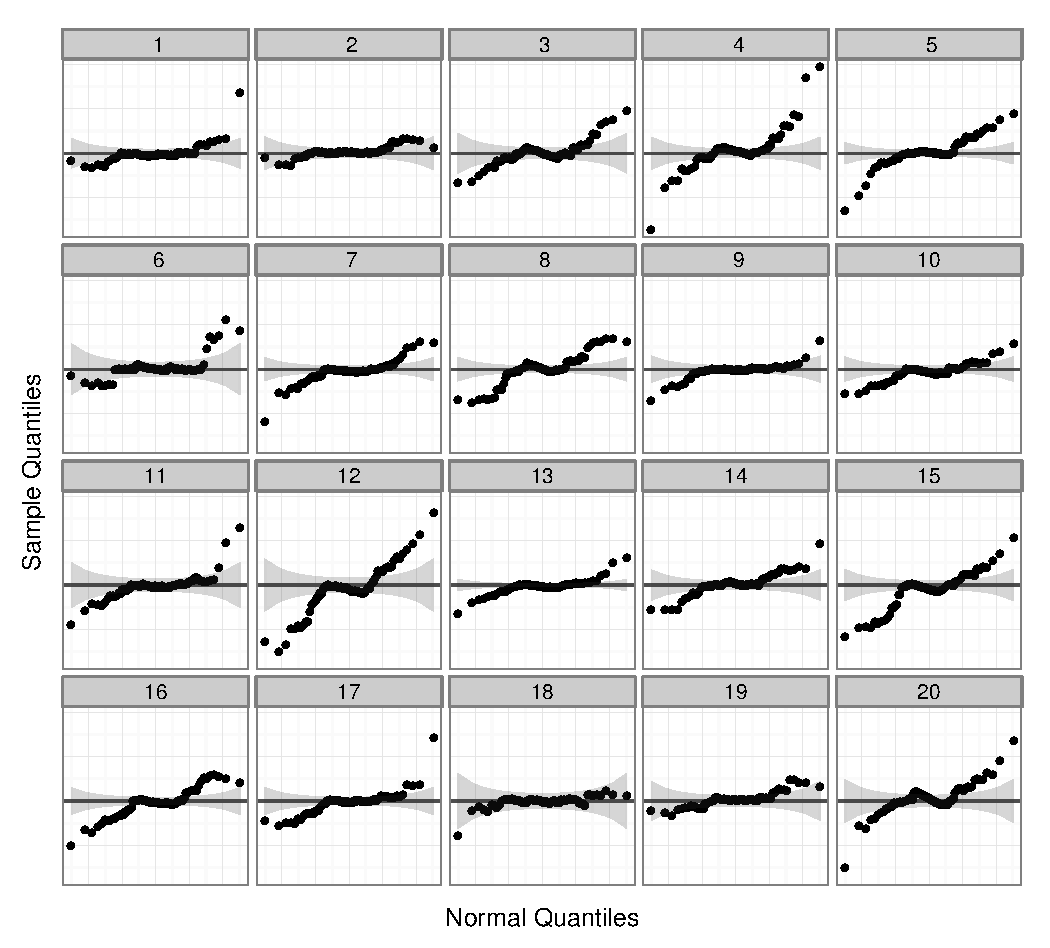
\includegraphics[width=0.9\textwidth]{qq-lineup-rot.pdf}%test.jpeg}%lineup-rslope.pdf}
	\caption{\label{fig:lineup-2} Lineup of detrended Q-Q plots for the random slope term in model~\eqref{eq:radon}. This plot shows the same data as the standard Q-Q plots of figure~\ref{fig:lineup}. Out of 22 evaluations, 11 participants picked panel \#$(3^2+3)$ as the most different from the set; another 4 participants chose panel \#$(2 \cdot 3^2)$. None of the participant picked the panel of the observed data.}
\end{figure}

\begin{table}[ht]
% latex table generated in R 3.1.0 by xtable 1.7-3 package
% Wed Jul 30 15:49:14 2014
\centering
\begin{tabular}{rrrrrrrrrrr}
  \hline
  & \multicolumn{9}{l}{response} \\
Q-Q type & 2 & 3 & 4 & 5 & 6 & 11 & 12 & 15 & 18 & 20 \\ 
  \hline
  Standard & 0 & 0 & 2 & 1 & 2 & 1 & 15 & 4 & 0 & 2 \\ 
  Detrended & 1 & 1 & 1 & 1 & 0 & 0 & 11 & 2 & 4 & 1 \\ 
   \hline
\end{tabular}
\caption{\label{tab:lpresults}Overview of user picks evaluating lineups in figures~\ref{fig:lineup} and \ref{fig:lineup-2} for the panel with the most pronounced difference. Both standard and detrended version of Q-Q plots show similar results with a definite preference for panel \#12.}
\end{table}

%----------------------------------------------------------------------------------
\section*{Supplementary Materials}
%----------------------------------------------------------------------------------

The following supplemental materials can be obtained online:

\begin{description}
\item[Simulation results:] The supplementary materials include the full simulation study discussed in Section~\ref{sec:simulation}. Additionally, the results of a simulation supporting the small simulation study discussed in Section~\ref{sec:ex} are presented and further show the need for alternative procedures to assess the distribution of the random effects.

\item[\texttt{R} script for figures and simulations:] The \texttt{R} code and data used to generate results discussed in this paper are available in the file \texttt{code\_supplement.zip}. 

\item[\texttt{R} package \texttt{HLMdiag}:] We have included the function to calculate the rotated random effects in the \texttt{R} package \texttt{HLMdiag}. The stable version of \texttt{HLMdiag} is available from the Comprehensive R Archive Network (CRAN, \url{http://cran.r-project.org/}) and the developmental version is available of github (\url{https://github.com/aloy/HLMdiag}).
\end{description}

%----------------------------------------------------------------------------------
%----------------------------------------------------------------------------------
\bibliographystyle{asa}
\bibliography{lcresid_bib}
%----------------------------------------------------------------------------------
%----------------------------------------------------------------------------------



\end{document}